%%%%%%%%%%%%%%%%%%%%%%%%%%%%%%%%%%%%%%%%%
% Beamer Presentation
% LaTeX Template
% Version 1.0 (10/11/12)
%
% This template has been downloaded from:
% http://www.LaTeXTemplates.com
%
% License:
% CC BY-NC-SA 3.0 (http://creativecommons.org/licenses/by-nc-sa/3.0/)
%
%%%%%%%%%%%%%%%%%%%%%%%%%%%%%%%%%%%%%%%%%

%----------------------------------------------------------------------------------------
%	PACKAGES AND THEMES
%----------------------------------------------------------------------------------------

\documentclass{beamer}
\mode<presentation> {

% The Beamer class comes with a number of default slide themes
% which change the colors and layouts of slides. Below this is a list
% of all the themes, uncomment each in turn to see what they look like.

%\usetheme{default}
%\usetheme{AnnArbor}
% %\usetheme{Antibes}
%\usetheme{Bergen}
%\usetheme{Berkeley}
%\usetheme{Berlin}
%\usetheme{Boadilla}
%\usetheme{CambridgeUS}
%\usetheme{Copenhagen}
%\usetheme{Darmstadt}
%\usetheme{Dresden}
%\usetheme{Frankfurt}
%\usetheme{Goettingen}
%\usetheme{Hannover}
%\usetheme{Ilmenau}
%\usetheme{JuanLesPins}
%\usetheme{Luebeck}
\usetheme{Madrid} %%%%
%\usetheme{Malmoe}
%\usetheme{Marburg}
%\usetheme{Montpellier}
%\usetheme{PaloAlto}
%\usetheme{Pittsburgh}
%\usetheme{Rochester}
%\usetheme{Singapore}
%\usetheme{Szeged}
%\usetheme{Warsaw}

% As well as themes, the Beamer class has a number of color themes
% for any slide theme. Uncomment each of these in turn to see how it
% changes the colors of your current slide theme.

%\usecolortheme{albatross}
%\usecolortheme{beaver}
%\usecolortheme{beetle}
%\usecolortheme{crane}
%\usecolortheme{dolphin}
%\usecolortheme{dove}
%\usecolortheme{fly}
%\usecolortheme{lily}
%\usecolortheme{orchid}
%\usecolortheme{rose}
%\usecolortheme{seagull}
%\usecolortheme{seahorse}
%\usecolortheme{whale}
%\usecolortheme{wolverine}

%\setbeamertemplate{footline} % To remove the footer line in all slides uncomment this line
%\setbeamertemplate{footline}[page number] % To replace the footer line in all slides with a simple slide count uncomment this line

%\setbeamertemplate{navigation symbols}{} % To remove the navigation symbols from the bottom of all slides uncomment this line
}

\usepackage{graphicx} % Allows including images
\usepackage{graphics}
\usepackage{booktabs} % Allows the use of \toprule, \midrule and \bottomrule in tables
\usepackage[english, french]{babel}  %support francais et anglais
\usepackage[utf8]{inputenc}
%\bibliographystyle{plainnat}
%\bibliography{cdansereau}


%----------------------------------------------------------------------------------------
%	TITLE PAGE
%----------------------------------------------------------------------------------------

\title[Connectivity for early diagnosis of AD]{Selection of multiscale functional brain connections for early diagnosis of Alzheimer's disease in multicentric studies} % The short title appears at the bottom of every slide, the full title is only on the title page

\author{Christian Dansereau} % Your name
\institute[DIRO] % Your institution as it will appear on the bottom of every slide, may be shorthand to save space
{
Université de Montréal \\ % Your institution for the title page
\medskip
%\textit{john@smith.com} % Your email address
}
\date{5 décembre 2014} % Date, can be changed to a custom date

\begin{document}

\begin{frame}
\titlepage % Print the title page as the first slide
\end{frame}

\begin{frame}
\frametitle{Overview} % Table of contents slide, comment this block out to remove it
\tableofcontents % Throughout your presentation, if you choose to use \section{} and \subsection{} commands, these will automatically be printed on this slide as an overview of your presentation
\end{frame}

%----------------------------------------------------------------------------------------
%	PRESENTATION SLIDES
%----------------------------------------------------------------------------------------

%------------------------------------------------
\section{Contexte général} 
%------------------------------------------------
%\begin{frame}
%\frametitle{Contexte général}


%The number of Canadians suffering from Alzheimer's disease (AD) is rapidly increasing, with tremendous social and economic impact. Despite the emergence of promising drugs, the recent clinical trials with demented patients have failed. Dementia however comes very late in the development of the disease, at a stage where the degeneration of neural tissues has likely gone beyond repair. In order to be efficient, therapies should be initiated in the decades predating dementia, in a preclinical stage where patients experience no or very mild symptoms (see chapter $1.1$). There are unfortunately no biomarker(s) that are currently predictive of AD in this preclinical stage, and could help identify the individuals that could benefit from such interventions. A promising technique is resting-state functional magnetic resonance imaging (rs-fMRI), which may be able to capture the early synaptic dysfunction seen in AD (see chapter $1.2$). I order to be able to apply statistical analysis and machine learning methods we 
%need to preprocess the data to remove as much as possible the effect of various artefacts (hardware and physiological). The preprocessing reduces the variability of the data and therefore provides more relevant and discriminative features (see chapter $1.3$). In order to further improve the statistical power of there analysis, multiple academic groups are collaborating to pool their dataset to increase the sample size of the study. Unfortunately the gain in sample size comes with a new source of variability introduced by the multicentric acquisition. Site-specific MRI set-ups may bias the fMRI measures, and I am thus developing procedures for inter-site normalization. Account for these sources of variance are important since they may bias the predictive potential of rs-functional connectivity in a multi-site, in line with this last assumption we want to quantify the robustness of the feature selection and classifier to multi-site acquisition (see chapter $1.4$).
%\end{frame}
%------------------------------------------------
%\begin{frame}
%\frametitle{Contexte général}
%With the objective of extracting meaningful information that could be used as biomarkers we are using connectivity measures usually based on the correlation of spontaneous fluctuations in neurovascular activity from pairs of brain regions, which have been shown to be sensitive to the development of the disease (see chapter $1.5$). However, with about $10^4$ recording sites in the gray matter and close to no knowledge on the early brain dysfunction in AD, there is an overwhelming number of $10^7$ possible connections to examine as a potential diagnostic we will therefore focus on the feature selection procedure and the stability of those selections in order to have consistent and sparse predictive features discriminative of the disease(see chapter $1.6$). The main outcome of this project will be a prediction pipeline for the data-driven identification of AD biomarkers in resting-state fMRI.
%
%\end{frame}
%------------------------------------------------
%\subsection{Maladie d'Alzheimer} 
%------------------------------------------------
\begin{frame}
\frametitle{Definition de la maladie d'Alzheimer}
\begin{itemize}
\item Maladie neurodégénérative incapacitante.
\item Cause la plus fréquente de démence chez l’homme (36M). 
\item Bases physiologiques encore mal comprises.
\end{itemize}
\end{frame}

% \begin{frame}
% \frametitle{Phases de la maladie d'Alzheimer}
% \begin{itemize}
% \item Phase pre-symptomatique (cognitivement normaux mais changement apparaise dans certaint cas )
% \item Phase prodromique (au moins un domaine cognitif) (MCI)
% \item Démence (atteinte sur plusieurs domaines) (incapable de fonctionner)
% \end{itemize}
% \end{frame}

\begin{frame}
\frametitle{Progression de la maladie d'Alzheimer}
\begin{figure}[H]
\begin{center}
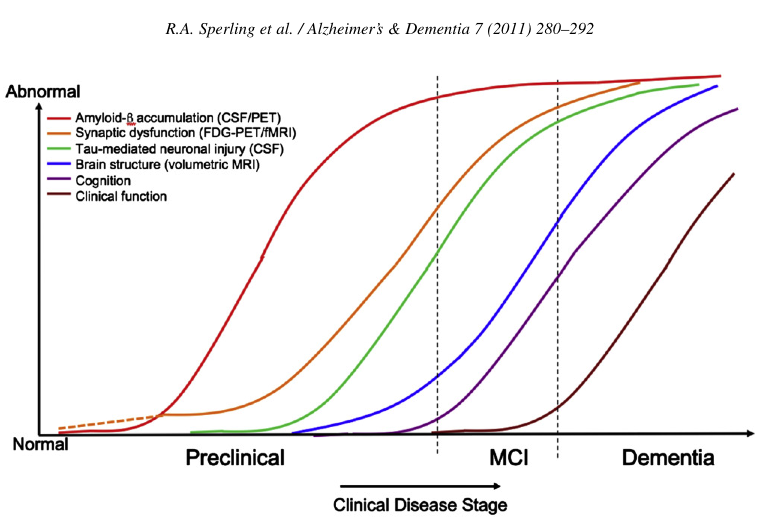
\includegraphics[scale=0.7]{../figures/ad_progression.png}
\end{center}
\label{fig_biomarker_model}
\end{figure}
\end{frame}

%------------------------------------------------
%\subsection{Imagerie par résonance magnétique fonctionnelle} 
%------------------------------------------------

\begin{frame}
\frametitle{Imagerie par résonance magnétique (IRM)}
\begin{figure}
\begin{center}
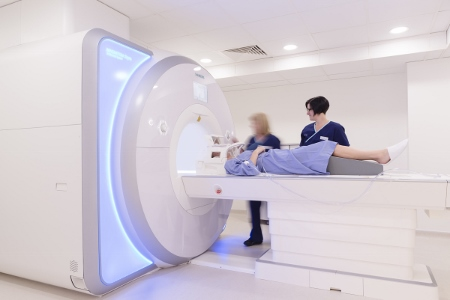
\includegraphics[width=0.7\linewidth]{../figures/scanner.jpg}
\end{center}
\end{figure}
\end{frame}


\begin{frame}
\frametitle{IRM fonctionnelle (IRMf)}
\begin{figure}[H]
\begin{center}
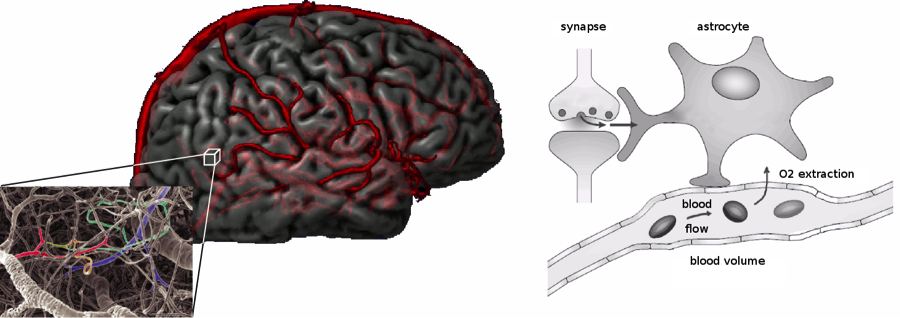
\includegraphics[width=\linewidth]{../figures/bold.png}
\end{center}
% \tiny{Representation of the brain and its vasculature (on the left) and a schematic view of the interaction between the effect of neuronal activity on local changes in blood oxygenation signal (BOLD) (on the right) (adapted from Heeger 2002).}
\tiny{Adapté de Heeger 2002.}

\end{figure}
\end{frame}
%------------------------------------------------
%\subsection{Prétraitement} 
%------------------------------------------------

\frame{
\frametitle{Connectivité au repos (resting-state)}
\begin{figure}
\pgfimage[width=0.8\linewidth]{fig_fcmri}\\
\tiny{Tiré de (Bellec, Springer 2011).}
\end{figure}
\tiny{Le cortex cingulaire postérieur est utilisé comme cible pour une carte de connectivité fonctionnelle individuelle en IRMf.}
}

% \begin{frame}
% \frametitle{Prediction et classification en AD}
% 
% \begin{itemize}
% \item Plusieurs études majeures ont été initié dans le but de prédire le développement de la maladie d’Alzheimer (prodromal et/ou asymptomatique)
% \item Objectif ultime étant une plateforme d’intervention thérapeutique (avec des médicaments spécifiques à la maladie)
% \item Presentement une très petite littérature rapporte des résultats en prédiction sur maladie d’Alzheimer.
% 
% \item Les seuls sont Jiang 2014 ($94\%$) (problème avec la cross-validation)
% ou Chen 2011 ($87\%$) et Dai 2014 ($80\%$) mais avec de très petits n (potentiel problème de généralisation)
% \end{itemize}
% \end{frame}

\frame{
\frametitle{Comparison between healthy subjects, patients with MCI and patients with a dementia of the AD type}
\begin{figure}
\pgfimage[width=0.7\linewidth]{fig_koch2012}\\
\tiny{A two sample $t$-test between healthy elderly subjects ($n=21$), patients with MCI ($n=17$) patients with a DAT ($n=15$), using various connexions within the default-mode network. Statistics corrected for multiple comparisons with the false-discovery rate ($q\leq 0.05$).\\From Koch et al., 2012, Neurobiology of aging, 466-478.}
\end{figure}
}

% \begin{frame}
% \frametitle{Connectivitée au repos}
% \begin{figure}
% \begin{center}
% \pgfimage[width=0.8\linewidth]{../figures/connectome.png}
% \end{center}
% \tiny{Bellec et al. Neuroimage 2006
% Functional connectome: on the left a representation of a functional parcellation, in the middle a region-level functional connectome representing the connectivity between each pair of region and on the right the connectivity map based on a region of interest extracted from the functional connectome.}
% \end{figure}
% \end{frame}



% \begin{frame}
% \frametitle{BOLD effect}
% \begin{figure}[H]
% \begin{center}
% 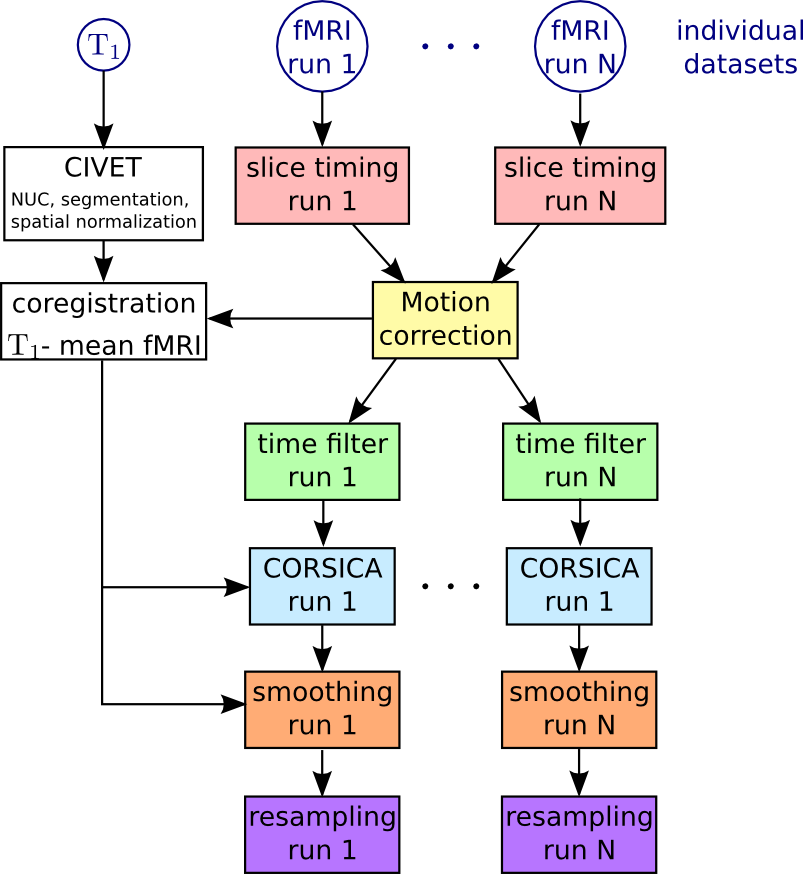
\includegraphics[scale=0.7]{../figures/fig_flowchart_fmri_preprocess.png}
% \end{center}
% \tiny{Schematic of the preprocessing pipeline including spatial and functional normalization (NIAK preprocessing pipeline \footnote{\url{http://www.nitrc.org/projects/niak/}}).}
% \label{fig_preprocessing}
% \end{figure}
% \end{frame}



%------------------------------------------------
%\subsection{Multi-site} 
%------------------------------------------------
% \begin{frame}
% \frametitle{Prétraitement}
% Importance de la normalisation des données pour l’observation de différences entre les groupes.
% \hfill\break
% Sources de bruit :
% \begin{itemize}
% \item Battement cardiaque, respiration, mouvement ...
% \item Normalisation spatiale (dans un espace commun)
% \end{itemize}
% \hfill\break
% Une chaine de traitements est utilisé pour dimimnuer le bruit structuré
% 
% %Normalization of the data is crucial to obtain a consistent and accurate classifier (Kotsiantis 2007). Therefore a particular attention is place on the correction and normalization procedure applied to the rs-fMRI data used in this study. A series of standard preprocessing steps is usually applied in an attempt to correct for various artefacts that would perturb the subsequent analysis. The BOLD effect associated with neuronal activity generally results in a relatively small fluctuation of the MR signal. Many factors can influence this signal. Among them,  the physiological activity associated mainly with respiration, cardiac pulsations and patient's motion are major contributors to the noise and are spatially spread everywhere within the brain volume. These sources of noise result in large correlations between BOLD signals of distant voxels. An other factor is the fact that we need a form of spatial normalization of the individual brains in order to perform analysis across subjects (due to anatomical 
% %variance among subjects), this spatial normalization (coregistration of the individual brains with an reference template) is necessary but can potentially be an other source of confound. Therefore, preprocessing methods were designed in an attempt to remove specifically the so-called structured noise and motion artefacts from the raw fMRI data. A schematic representation of the preprocessing pipeline.
% \end{frame}




% \frame{
% \frametitle{AD and connectivity}
% \begin{figure}
% \pgfimage[width=0.8\linewidth]{../figures/fig_buckner2009}\\
% \end{figure}
% \tiny{From Buckner et al., 2009}
% }


%------------------------------------------------
%\subsection{Prediction et classification} 
%------------------------------------------------

%In the past few years, several major studies have been initiated that have aimed to predict who will develop AD at the prodromal or even asymptomatic stage, with the ultimate goal of providing a platform for therapeutic intervention with disease-modifying therapies. Many of these studies were designed to evaluate the role of neuroimaging and chemical biomarkers in assessing and predicting progression in individuals without cognitive impairment and in individuals with MCI.
%A very small literature currently reports findings on AD using rs-fMRI and they usually have outstanding performance like Jiang2014 ($94\%$). Unfortunately, the authors of this study performed a 10-fold cross-validation which did not include the feature selection process, which potentially lead to overestimation of the real accuracy. The rest of published studies have mainly used leave one out cross-validation and small sample size, which raises some concern with regards to the generalization ability of those trained predictors, e.g. Chen2011 ($87\%$), Dai2014 ($80\%$)).

%\subsection{Importance of preprocessing to improve classification}
%Preprocessing and normalization of the source data is a crucial point that may affect greatly the resulting classification or potential outcome measures. Moreover the introduction of multicentric data in the classification will render the task even more difficult, Nevertheless, a multi-site cohort helps test generalizability of the results across different samples, making it more likely that connections identified as predictive of a disease state indeed reflect generic traits of the pathology rather than particularities of a single dataset.

%\subsection{High dimensionality problem}
%In rs-fMRI, we obtain signal from brain activity at the voxel level representing more than $10^4$ voxels in the gray matter cortex, where the vast majority of the neurons are located. Although preprocessed, these data continue to have a lot of variance and we need to identify functional organisation more meaningful in term of clinical interpretation as well as an improved representation of the feature space that enhance the characterization of the functional modules. We can commonly extract functionally and clinically meaningful network features using principal component analysis (PCA) Zhong2009, independent component analysis (ICA) McKeown1998, various clustering algorithms such as k-means Baumgartner1998, hierarchical clustering Cordes2002, normalized cut-graph Heuvel2008, self-organizing maps and neural gas Meyer-Baese2004. Once we have functional parcels of the brain it is important to find the right metric to evaluate the connectivity between regions of the brain at the individual level. The most 
%common metric use in the field of connectivity is the Pearson's correlation coefficient between the time series associated with a pair of regions.

%\subsection{Feature selection}
%Feature selection is often a critical step prior to any learning algorithm. The selection reduces the computational complexity of learning algorithms and exposes potentially clinically meaningful information. In many cases, this process can also improve the prediction accuracy by removing redundant and irrelevant information. Therefore feature selection is an important step in effective learning of large data sets. The features selection methods are usually organized into two categories: filter methods and wrapper methods Kotsiantis2007. The filter method evaluates the relevance of features by looking only at the properties of the data without any knowledge on the classification labels. The wrapper method assesses the goodness a feature subset using the performance of a learning algorithm. The lack of reproducibility of reported markers (subset of features) is one of the main obstacle for the adoption of such marker in a clinical setup. If the marker is indeed discriminative of the pathology or of its 
%progression we would expect the same features to be selected and exhibit similar performance across various studies. 

%\subsection{Classification}
%Machine learning methods have become very popular to classify functional brain images Costafreda2009,Fu2008,Hahn2011,Marquand2008,Nouretdinov2011, for example to discriminate them between healthy and diseased populations. The most popular machine learning techniques in fMRI arguably is support vector machine (SVM) Cortes1995 which has been used in the past to categorize individual structural or functional brain images by differentiation of images from two groups (e.g. patient/control or male/female) Lao2004, Fan2005, Mourao-Miranda2005, Kawasaki2007. 
%A second widely used method is linear discriminant analysis (LDA) classifier; the main advantage of LDA is the ability to easily include confounding effects in the decision model, such as the inter-site difference in average connectivity measures.

%\end{frame}
% \frame{
% \frametitle{Prediction et classification en AD}
% \begin{itemize}
% \item Prétraitement des données peuvent influencer la prédiction.
% \item Métrique utilisée, autre que la correlation.
% \item Manque de reproductibilité entre sites est l’un des principaux obstacles de l’adoption de ce genre de biomarqueur en un contexte clinique.
% \item Réduction des données dans un espace avec un sens clinique.
% 
% \end{itemize}
% 
% }


%------------------------------------------------
%\subsection{Objectives} % A subsection can be created just before a set of slides with a common theme to further break down your presentation into chunks
%------------------------------------------------
\begin{frame}
\frametitle{Objectifs}
\begin{enumerate}
\item \emph{L'analyse de données en IRMf n'est pas optimisée pour des populations âgées (CNE, pMCI, pDAT).}\\ \textbf{Objectif 1:} Optimiser la chaine de traitements des données d'IRMf pour ces populations. 
\item \emph{La collecte de grands échantillons passe par l'acquisition de données dans plusieurs centres d'imagerie.}\\ \textbf{Objectif 2:} Evaluer la faisabilité d'études multicentriques en IRMf.
\item \emph{De nombreuses mesures peuvent être générées en IRMf}.\\ \textbf{Objectif 3:} Élaborer un algorithme d'identification de biomarqueurs de la maladie d'Alzheimer.
\end{enumerate}
\end{frame}

%------------------------------------------------
\section{Optimisation des étapes de prétraitement} %Scrubbing and motion artefact correction
%------------------------------------------------

\frame{\sectionpage}

\begin{frame}
\frametitle{Correction des artefacts de mouvement}
Les mouvements de la tête sont inévitables et présentent l’un des plus grands problèmes en IRMf.
\hfill\break
\begin{itemize}
\item Possibilité de réaligner les déplacements de la tête.
\item Ne corrige pas les artefacts induits dans le signal par des inhomogénéités du champ magnétique.
\item Le mouvement est plus important/fréquent chez les populations âgées. 
\end{itemize}
\end{frame}


\begin{frame}
\frametitle{Objectifs étude 1}
\begin{itemize}
\item Évaluer la quantité de mouvement chez les populations âgées ainsi que celles avec un début de démence.
\item Évaluer l’impact du prétraitement sur la connectivité.
\item Évaluer l’impact du prétraitement sur notre capacité à détecter un effet.
\end{itemize}
\end{frame}

% \begin{frame}
% \frametitle{Étapes du prétraitement}
% \begin{enumerate}
% \item Slice timing correction
% \item rigid-body motion estimation
% \item Coregistration of the functional in reference space
% \item resampling in stereotaxic space
% \item Regression of confounds (remove structures noise)
% \item Spatial smoothing
% \end{enumerate}
% %The basic steps are as follow: (1) correction for slice timing differences due to delay in acquisition sampling; (2) rigid-body motion estimation for within and between runs, motion correction operates by selecting one functional volume as a reference to align all other functional volumes. Most head motion algorithms describe head movement by 6 parameters, three translation (displacement) parameters and rotation parameters and are appropriate to characterize motion of rigid bodies (see Figure \ref{fig_motion_estimation}); (3) Coregistration of the functional data in a reference space; (4) resampling of the functional data in the stereotaxic space (references brain used as a common space between subjects); (5) regression of confounds in order to remove spatially structured noise on the fMRI time-series. The confounds are the slow time drift, high frequency noise signal, motion parameters, the average signal white matter as well as the average signal of the ventricles (containing cerebrospinal fluid CSF a 
% %frequent source of noise and artefact). Some groups have suggested that these corrections are not sufficient to remove motion artefact and propose some additional corrective procedure (detailed in Chapter 2); and (6) the spatial smoothing is usually applied using a Gaussian blurring kernel to improve signal to noise ratio (SNR)
% \end{frame}


\begin{frame}
\frametitle{Estimation du mouvement}
\begin{figure}
\begin{center}
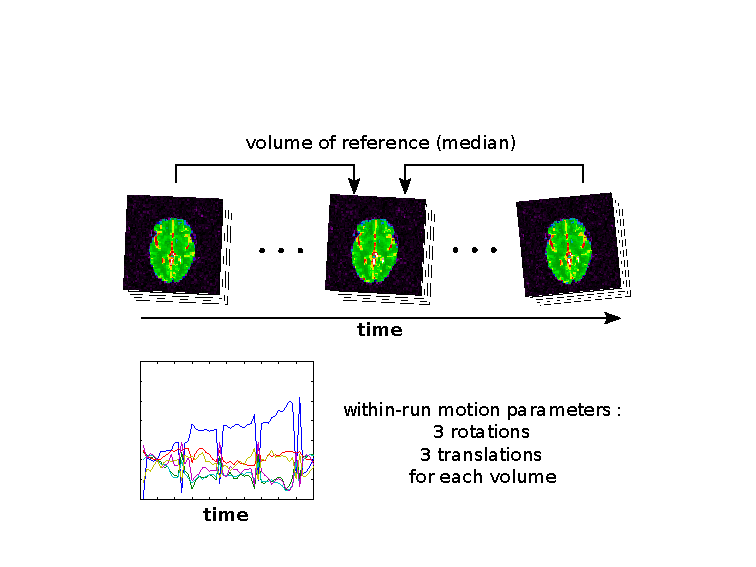
\includegraphics[scale=0.9]{../figures/motion_estimation.pdf}
\end{center}
\tiny{%Motion estimation based on rigid-body motion estimation of the functional volumes, the procedure provide 6 motion parameters for each volume (3 translation and 3 rotation) Schematic of the preprocessing pipeline including spatial and functional normalization 
(from Chaine de prétraitement du ``Neuroimaging Analysis Kit'' (NIAK) \footnote{\url{http://www.nitrc.org/projects/niak/}}).}
\label{fig_motion_estimation}
\end{figure}
\end{frame}



%Head motion is probably the most severe problem in fMRI studies, although it cannot be avoided. The quality of the fMRI data is strongly affected by the presence of head motion. As previously mention, a number of publications have proposed post-hoc correction in order to reduce head motion artefact. Although head motion can be corrected in the image space, displacement of the head reduces the homogeneity of the magnetic field, which is fine-tuned prior to functional scans for a given head position. Since head displacements lead to non-optimal tuning, motion artefacts are not fully removed even after perfect realignment of successive functional volumes in image space. The impact of motion and the method available to reduce its effect on functional connectivity thus need to be carefully evaluated. Typically subjects with average motion over 3 mm are excluded from the analysis. A first popular technique to reduce motion artifact is global signal correction (GSC), which consists of regressing the average of all 
% the time-series in the brain. This technique has raised a number of concerns due to the potential artificial introduction of anti-correlation in the data (Fox2009,Murphy2009, Saad2012, Carbonell2014, Power2014). Another corrective measure is the CompCor method \citep{Behzadi2007} that regresses out the $n$ first components of a principal component analysis (PCA) on the time-series of the white matter and cerebrospinal fluids voxels. As no signal of neuronal origin are expected in such areas, the CompCor method was suggested to provide a compact representation of the structured noise present in an fMRI dataset. Both GSC and CompCor are global corrections, which are not specific to motion correction. The GSC in particular incorporates signal from the grey matter regions. Power and colleagues showed in 2012 that spurious but systematic correlations in fc-MRI arise from subject motion even at levels previously regarded as insignificant  (variation smaller than $1$ mm / degree in motion parameters) and are 
% not adequately removed by common functional connectivity processing steps. Power et al. 2012 suggested using a method called ``scrubbing'' (or censoring) in order to reduce motion-related bias from  fMRI time-series. With the scrubbing method, the frames with motion level above a certain threshold are simply removed from the time-series. The metric used to quantify the level of motion from one frame to the other is called framewise displacement (FD). It is calculated as the sum of the absolute values of the differentiated realignment parameters estimated at every time point, giving an approximate conversion of rotation parameters ($\alpha_{i},\beta_{i},\gamma_{i}$) in a unit equivalent to a translation in millimeters on a sphere of radius 50mm and translation parameters ($d_{ix},d_{iy},d_{iz}$) for the other rigid body parameters. The main limitation of the scrubbing method is the loss of time-points, which can lead to subjects loss due to an insufficient number of time point remaining after scrubbing 
% correction. The question is therefore to evaluate if the trade-off between data loss and quality is detrimental or beneficial to statistical power. I have recently published results concerning this issue (Dansereau et al. 2014) (published proceeding and manuscript in preparation). In this work we aimed to (1) characterize the impact of motion on rs-fMRI in cognitively normal elderly (CNE)  participants as well as patients with mild cognitive impairment (pMCI) and dementia of the Alzheimer's type 0.5-No (pDAT), and, (2) evaluate how the scrubbing impacts the differences in connectivity between groups (CNE, pMCI, pDAT).

\begin{frame}
\frametitle{Résumé de la quantité de mouvement}
Mesure dite de ``frame displacement'' (FD). 
\begin{equation}
    FD_{i} = \vert \triangle d_{x}(t) \vert + \vert \triangle d_{y}(t) \vert + \vert \triangle d_{z}(t) \vert + \vert \triangle r_x(t) \vert + \vert \triangle r_y(t) \vert + \vert \triangle r_z(t) \vert,
\end{equation}
\begin{equation}
  r_x(t) = 50\left(\frac{2\pi\alpha_x(t)}{360}\right),
\end{equation}
avec 
\begin{itemize}
 \item ($d_x(t),d_{y}(t),d_{z}(t)$) paramètres de translation (mm),
 \item ($\alpha_x(t),\alpha_y(t),\alpha_z(t)$) paramètres de rotation (degrés),
 \item $\triangle$ la différence entre l'instant $t$ et $t-1$.
\end{itemize}
\end{frame}


%\frame{
%\frametitle{Correction}
%Approches existantes:
%\begin{itemize}
%\item Régression des paramètres du mouvement (3 translations et 3 rotations)
%\item Global signal correction (GSC)
%\item CompCor
%\item Scrubbing
%\end{itemize}
%}


\frame{
\frametitle{Prétraitement}
%Les étapes décrites précédemment ont été appliquées
%\hfill\break
\begin{itemize}
\item Prétraitement standard (sans scrubbing)
\item Avec scrubbing ($FD>0.5$)
\item Avec scrubbing ($FD>0.2$)
%\item Régression de variable de non-intérêt (standard + GSC)
%\item Régression de variable de non-intérêt (standard + CompCor)
\end{itemize}
\hfill\break
Minimum de 50 volumes restant.
}

\frame{
\frametitle{Jeux de données}
Ce projet provient de l’agrégation de plusieurs jeux de données (5 études différentes)
\hfill\break
ADNI2 et 4 études basées à Montréal (total: 313 sujets)
\begin{itemize}
\item 126 CNE participants (51M, âge = 57-94)
\item 133 pMCI (70M, âge = 55-89) 
\item 54 pDAT (22M, âge = 55-88)
\end{itemize}
\hfill\break
Jeux de données de référence: ``1000 functional connectome project''
\begin{itemize}
\item 355 jeunes adultes sains (CNY) (150M, âge = 18-46)
\end{itemize}
%This project was based on a real dataset with fMRI data acuquired in different settings. The dataset included 313 elderly adults agregated across 5 independent studies:the ADNI2 study and 4 other studies based in Montreal, Canada. The dataset included three different clinical cohorts, for a grand total of 126 CNE participants (51 males, age range = 57-94 yrs), 133 patients with MCI (70 males, age range = 55-89 yrs), and 54 patients with DAT (22 males, age range = 55-88 yrs). We also included 355 cognitively normal young adults (CNY) from the 1000 functional connectome project (150 males, age range = 18-46 yrs) as a reference dataset (Biswal et al. 2010). This project was approved by the local ethics review board.
}


%\frame{
%\frametitle{Revue de la littérature: Alzheimer's disease and resting-state fMRI}
%Revue de la littérature pour sélectionner des connexions rapportées comme étant impactées par la malade d’Alzheimer
%\hfill\break
%Majorité des études comporte peu de sujets($n\sim20$).
%\hfill\break
%Focaliser notre attention sur le mode par défaut et sélectionner 6 articles 
%\begin{enumerate}
%\item Utilise un ou des points germe dans le DMN.
%\item Étudie la connectivité fonctionnelle au repos en démence du type Alzheimer.
%\item Contient des tables de résultat avec les coordonnées stéréotaxique.
%\end{enumerate}

%We performed a literature review to select candidate connections that have been shown to be prominently impacted in Alzheimer's disease. There is no single authoritative reference on the effect of a DAT on rs-fMRI connectivity, and the field has been dominated thus far by studies with small samples (n\textasciitilde20) and limited statistical power, see \cite{Sheline2013} for a recent review. Because the DMN has been most extensively studied, we decided to focus on this network and to run a meta-analysis on six papers that 
%(1) used some analogue of seed-based connectivity maps in resting-state fMRI using one or multiple seeds in the DMN 
%(2) investigated abnormalities in resting-state functional connectivity in patients suffering of a dementia of the Alzheimer's type and 
%(3) provided tables of coordinates in stereotaxic space for the results.
%}

% The datasets were analysed using the NeuroImaging Analysis Kit (NIAK1 ) version
% 0.12.14, under CentOS version 6.3 with Octave2 version 3.8.1 and the Minc toolkit3 ver-
% sion 0.3.18. Analyses were executed in parallel on the "Mammouth" supercomputer4 ,
% using the pipeline system for Octave and Matlab (Bellec et al. 2012), version 1.0.2.
% Brain map visualizations were created using MRICron software (Rorden et al. 2007).
% Each fMRI dataset was corrected of inter-slice difference in acquisition time and the pa-
% rameters of a rigid-body motion was estimated for each time frame. Rigid-body motion
% was estimated within as well as between runs, using the median volume of the first run
% as a target. The median volume of one selected fMRI run for each subject was coregis-
% tered with a T1 individual scan using Minctracc (Collins et al. 1998), which was itself
% non-linearly transformed to the Montreal Neurological Institute (MNI) template (Fonovet al. 2011) using the CIVET pipeline (Zijdenbos et al. 2002). The MNI symmetric tem-
% plate was generated from the ICBM152 sample of 152 young adults, after 40 iterations
% of non-linear coregistration. The rigid-body transform, fMRI-to-T1 transform and T1-
% to-stereotaxic transform were all combined, and the functional volumes were resampled
% in the MNI space at a 3 mm isotropic resolution. The ’scrubbing’ method of (Power et al.
% 2012), was used to remove the volumes with excessive motion with three cut-offs points:
% no scrubbing (FD \≥ 0), FD \≥ 0.5 and FD \≥ 0.2. A minimum number of 50 unscrubbed
% volumes per run, corresponding to ∼ 125 s of acquisition for a TR of 2.5 seconds, was
% then required for further analysis. For this reason, some subjects were rejected from the
% subsequent analyses: 11 CNE, 13 pMCI and 3 pDAT for a scrubbing at FD ≥ 0.5 and
% 83 CNE 95 pMCI and 39 pDAT for a scrubbing at FD \≥ 0.2 (see table 2.I). The fol-
% lowing nuisance parameters were regressed out from the time series at each voxel: slow
% time drifts (basis of discrete cosines with a 0.01 Hz high-pass cut-off), average signals
% in conservative masks of the white matter and the lateral ventricles as well as the first
% principal components (95\% energy) of the six rigid-body motion parameters and their
% squares (Lund et al. 2006),(Giove et al. 2009). The fMRI volumes were finally spatially
% smoothed with a 6 mm isotropic Gaussian blurring kernel.

% 
% \frame{
% \frametitle{Retention}
% \begin{table}
% \begin{center}
% 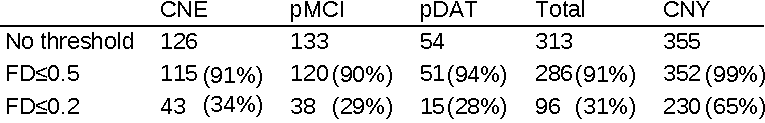
\includegraphics[width=0.75\linewidth]{../figures/table_retention.pdf}
% \end{center}
% \tiny{Retention rate for CNY, CNE, pMCI and pDAT at various scrubbing levels (standard, scrubbing $FD>0.5$ and scrubbing $FD >0.2$).}
% \label{tab_retention}
% \end{table}
% }

\frame{
\frametitle{Distribution du FD}
\begin{figure}
\begin{center}
\pgfimage[width=0.9\linewidth]{../figures/figure_fd_distrib.pdf}
\end{center}
\tiny{Distribution du FD pour chaque groupe (Dansereau et al. article en préparation)
%Distribution of the frame displacement (FD) for 3 groups (CNE, pMCI, pDAT) when scrubbing was applied at various levels (no scrubbing, scrubbing of $FD>0.5$ and scrubbing of $FD>0.2$). The boxplot on the right showed the distribution of FD with their associated statistical differences $t$-test (marked with a {\bf *} for a $p<0.05$).
}
\end{figure}
}

\frame{
\frametitle{Impact du prétraitement}
\begin{figure}
\begin{center}
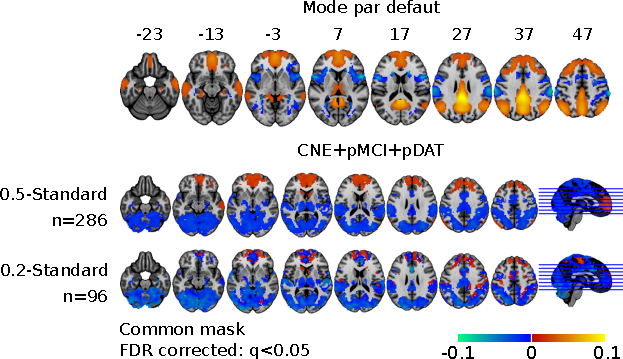
\includegraphics[width=\linewidth]{../figures/figure_comp1.pdf}
\end{center}
\tiny{Différence de connectivité entre stratégies de prétraitement (Dansereau et al., manuscript en préparation)
%Differences in functional connectivity for the default mode network (seed in the PCC). Differences in connectivity between all the groups pooled together (CNE, pMCI, pDAT) with scrubbing ($FD>0.5$ and $FD>0.2$), CompCor, and GSC. The mask used depicts only significant result of the $t$-test (FDR correction $q<0.05$) only the two scrubbing procedures use the union of their respective mask (common mask).
}
\label{fig_scrubbimpact}
\end{figure}
}

% \frame{
% \frametitle{Réseau du mode par défaut}
% \begin{figure}
% \begin{center}
% 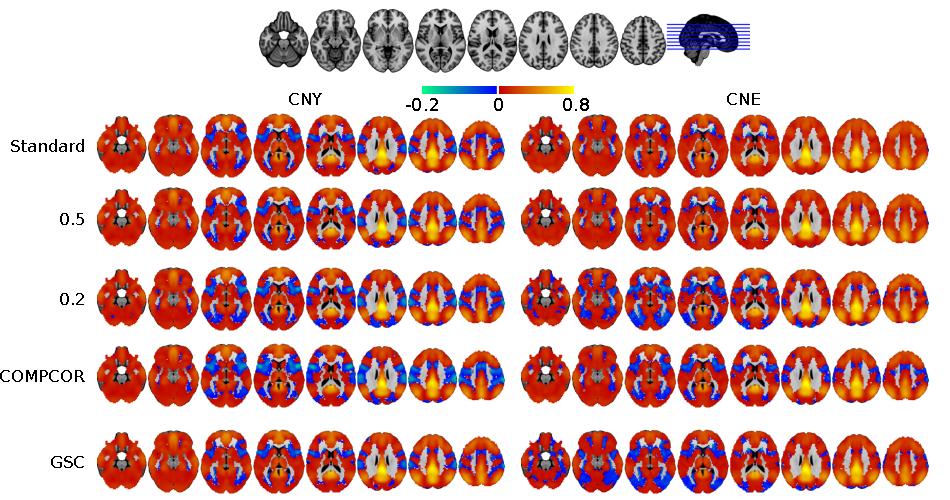
\includegraphics[width=\linewidth]{../figures/dmn_cny_cne.pdf}
% \end{center}
% \tiny{ Overlay of the average default mode network (DMN) with various preprocessing strategies for CNY and CNE populations on the ICBM 152 anatomical atlas. Seed based maps with a seed in the PCC using Fisher z transform of the Pearson's r correlation between the average time series of each network.
% }
% \label{fig_avg_dmn}
% \end{figure}
% }

% \frame{
% \frametitle{Impact du prétraitement}
% \begin{figure}
% \begin{center}
% 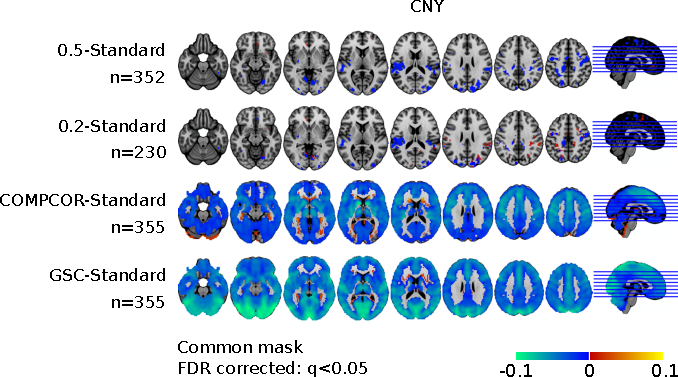
\includegraphics[width=\linewidth]{../figures/figure_comp_cny.pdf}
% \end{center}
% \tiny{
% {Differences in functional connectivity for the default mode network (seed in the PCC). Differences in connectivity between all the CNY with scrubbing ($FD>0.5$ and $FD>0.2$), CompCor, and GSC. The mask used depict only significant result of the $t$-test (FDR correction $q<0.05$) only the two scrubbing procedures use the union of there respective mask (common mask).}
% }
% \label{fig_sup_scrubbimpact_cny}
% \end{figure}
% }

%\frame{
%\frametitle{Impact du pretraitement sur chaque groupe}
%\begin{figure}
%\begin{center}
%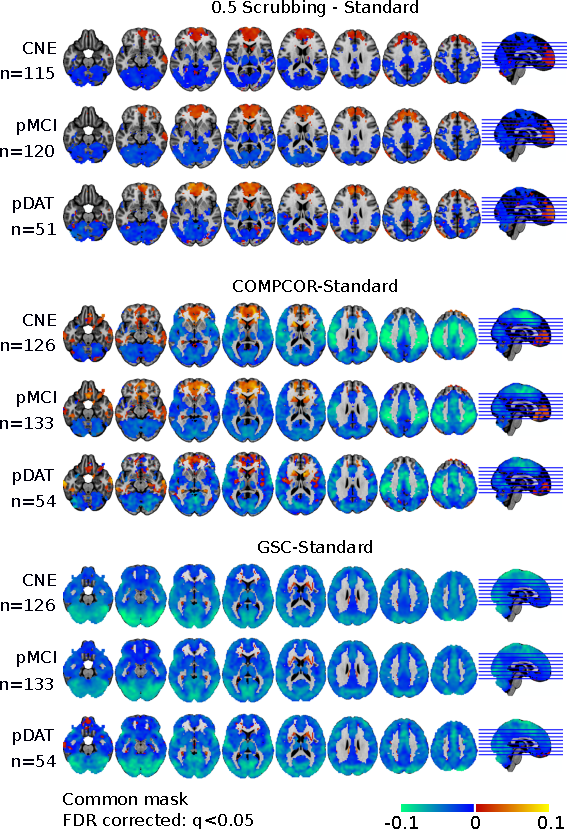
\includegraphics[width=0.40\linewidth]{../figures/scrubbing_impact_cne_mci_dat_all.pdf}
%\end{center}
%\tiny[Impact of preprocessing on each group]{
%{Differences in functional connectivity for the default mode network (seed in the PCC). Differences in connectivity for each group (CNE, pMCI, pDAT) compared to baseline (standard preprocessing) with and without scrubbing ($FD>0.5$), CompCor, and GSC (FDR correction $q<0.05$) for all voxels showing a significant effect in at least one of the contrast.}
%}
%\label{fig_sup_impact_on_groups}
%\end{figure}
%}

% \frame{
% \frametitle{Impact du pretraitement sur contraste pDAT-CNE}
% \begin{figure}
% \begin{center}
% 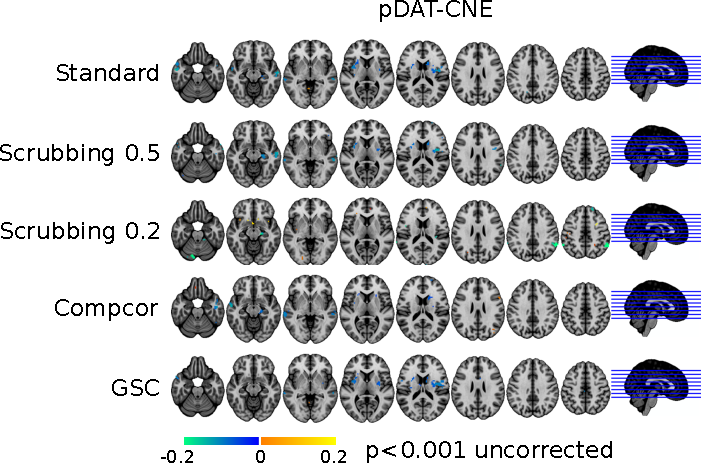
\includegraphics[width=0.80\linewidth]{../figures/scrubbing_impact_pDAT-CNE.pdf}
% \end{center}
% \tiny[Scrubbing impact on group differences]{ Impact of preprocessing on connectivity differences between the pDAT and CNE groups. Connectivity differences between DMN ($t$-test $p<0.001$ uncorrected) computed with various preprocessing strategies (standard, scrubbing (0.5 and 0.2), CompCor and GSC).The maps are represented on top of the ICBM 152 anatomical atlas.
% }
% \label{fig_impact_pDAT-CNE}
% \end{figure}
% }

%\frame{
%\frametitle{Impacte du pretraitement sur contraste pDAT-pMCI}
%\begin{figure}
%\begin{center}
%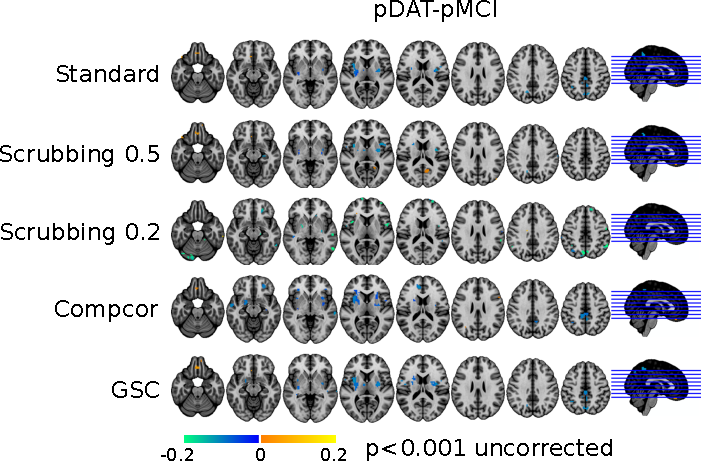
\includegraphics[width=0.60\linewidth]{../figures/scrubbing_impact_pDAT-pMCI.pdf}
%\end{center}
%\tiny{ Impact of preprocessing on connectivity differences between the pDAT and pMCI groups. Connectivity differences between DMN ($t$-test p<0.001 uncorrected) computed with various preprocessing strategies (standard, scrubbing (0.5 and 0.2), CompCor and GSC).The maps are represented on top of the ICBM 152 anatomical atlas.
%}
%\end{figure}
%}

%\frame{
%\frametitle{Impacte du pretraitement sur contraste pMCI-CNE}
%\begin{figure}
%\begin{center}
%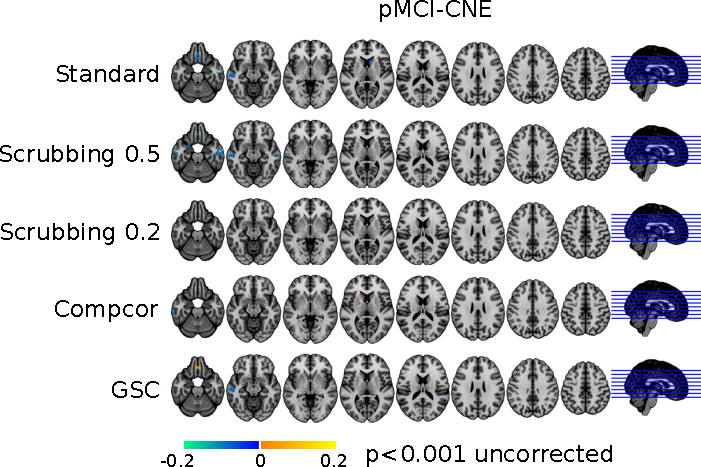
\includegraphics[width=0.60\linewidth]{../figures/scrubbing_impact_pMCI-CNE.pdf}
%\end{center}
%\tiny{ Impact of preprocessing on connectivity differences between the pMCI and CNE groups. Connectivity differences between DMN ($t$-test p<0.001 uncorrected) computed with various preprocessing strategies (standard, scrubbing (0.5 and 0.2), CompCor and GSC).The maps are represented on top of the ICBM 152 anatomical atlas.
%}
%\end{figure}
%}

\begin{frame}
\frametitle{Estimation de la sensibilité de détection}
\begin{itemize}
\item Différences inter-groupes (pDAT-CNE).
\item 10 paires de connexions reproductibles et impactées par la maladie sont sélectionnées sur la base de la littérature.
\item Modélisation (FD, âge, sexe) dans un GLM. Combinaison inter-sites par METAL.
\item Significativité des résultats obtenue avec un test $t$ de Student.
\item La sensibilité du test est évaluée en sous-échantillonnant 70\% du jeu de données ($B=10^4$ échantillons aléatoire).
\item Pour chaque échantillon $b$, on a une $p$-value $p^{*}_b$.
\item La sensibilité de la détection est donc estimée par la probabilité que $p^{*}_b$ soit inférieur à $0.05$.
\begin{equation}\label{Detection power}  
    \frac{1}{B}\sum\limits_{b=1}^B\left(p^{*}_b\leq0.05\right).
\end{equation}
\end{itemize}

\end{frame}


\frame{
\frametitle{Connexions selectionées}
\begin{figure}
\begin{center}
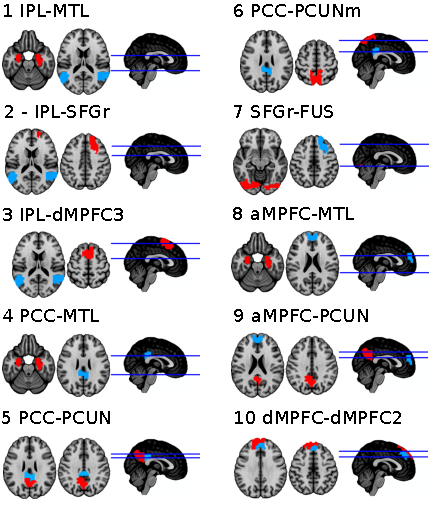
\includegraphics[width=0.5\linewidth]{../figures/p2p_seeds.pdf}
\end{center}
\tiny{Paires de connexions revue de littérature (Dansereau et al. article en préparation)
%On the Left: Seeds from 10 point-to-point connections. PCC (posterior cingulate cortex), PCUN (precuneus), dMPFC (dorsomedial prefrontal cortex), dMPFC2 (dorsomedial prefrontal cortex2), IPL (inferior parietal lobule), SFGr (right superior frontal gyrus), aMPFC (anterior medial prefrontal cortex), PCUNm (precuneus motor), dMPFC3 (dorsmedial prefrontal cortex3), MTL (Mesial temporal lobe). On the right: Detection power of group differences for 3 preprocessing strategy (standard, scrubbing $FD>0.5$ and scrubbing $FD >0.2$). The detection power is computed using a $t$-test of each connection ($p<0.05$) replicated $B=10^4$ times using random subsamples of 70\% of each group. Explanatory variables included age and gender and a multi-site bias correction are applied.
}
\label{fig_p2p}
\end{figure}
}


\frame{
\frametitle{Pouvoir de détection avec scrubbing}
\begin{figure}
\begin{center}
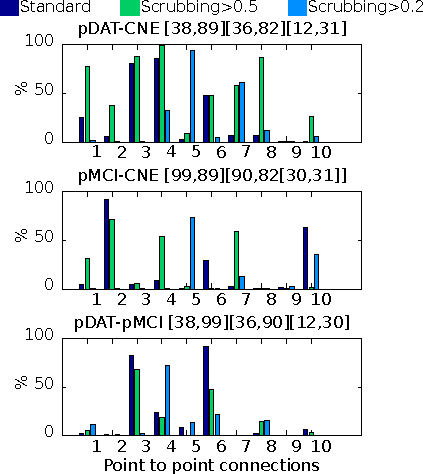
\includegraphics[width=0.8\linewidth]{../figures/p2pdetection.png}
\end{center}
\tiny{(Dansereau et al. article en préparation)
%On the Left: Seeds from 10 point-to-point connections. PCC (posterior cingulate cortex), PCUN (precuneus), dMPFC (dorsomedial prefrontal cortex), dMPFC2 (dorsomedial prefrontal cortex2), IPL (inferior parietal lobule), SFGr (right superior frontal gyrus), aMPFC (anterior medial prefrontal cortex), PCUNm (precuneus motor), dMPFC3 (dorsmedial prefrontal cortex3), MTL (Mesial temporal lobe). On the right: Detection power of group differences for 3 preprocessing strategy (standard, scrubbing $FD>0.5$ and scrubbing $FD >0.2$). The detection power is computed using a $t$-test of each connection ($p<0.05$) replicated $B=10^4$ times using random subsamples of 70\% of each group. Explanatory variables included age and gender and a multi-site bias correction are applied.
}
\label{fig_p2p}
\end{figure}
}

\frame{
\frametitle{Conclusions étude 1}
\begin{itemize}
\item Moins de données de meilleure qualité sont préférables à plus de données bruitées.
\item Prétraitement avec scrubbing à 0.5 pour les populations âgées, plutôt que 0.2 (seuil recommandé pour jeunes adultes).
\item Les techniques actuelles permettent de réduire mais pas d'effacer l'impact du mouvement.
\item Travail en cours: (1) précision de la prédiction plutôt que sensibilité. (2) approche METAL plus agressive.
\end{itemize}
}
% \frame{
% \frametitle{Pouvoir de detection avec GSC et CompCor}
% \begin{figure}[H]
% \begin{center}
% 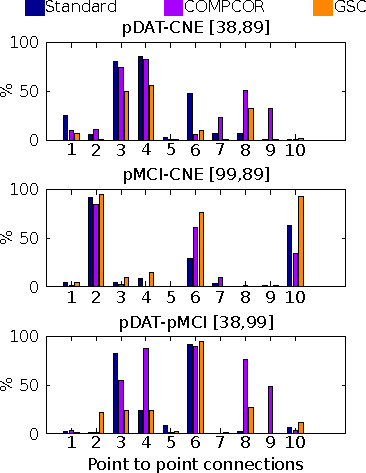
\includegraphics[width=0.5\linewidth]{../figures/p2pdetection_gsc_compcor.pdf}
% \end{center}
% \tiny[Detection power with CompCor and GSC]{
% Detection power of group differences for 3 preprocessing stategy (standard, CompCor and GSC)..
% }
% \label{fig_sup_p2p_gsc_compcor}
% \end{figure}
% }	

%------------------------------------------------
\section{Étude de connectivité multicentrique en IRMf} %Feasibility of multi-centric fMRI connectivity studies of Alzheimer's disease
\frame{\sectionpage}
\begin{frame}
\frametitle{Multi-sites}
Le nombre de sujets augmente mécaniquement la puissance statistique (sensibilité) d’une étude, ce qui peut être réalisé rapidement au moyen d'une étude multicentrique.
\begin{itemize}
\item Académique (ex. 1000 functional connectome, ADNI).
\item Pharmaceutique (essai clinique).
\end{itemize}

Source de variance: 
\begin{itemize}
\item variance d'acquisition (marque et modèle du scanneur)
\item contexte de l'expérience (instruction au participant, caractéristiques des populations locales)
\item variance de l'environnement (son, température).
\end{itemize}
\end{frame}
%(3) the sample size, i.e. the number of subjects in the study . This last factor is usually the only one controlled by the investigator, hence why an increasing number of researchers share multicentric, sometimes multiprotocol, data suitable to statistical analysis. In research it is very difficult to obtain a grant large enough to scan a cohort larger than ~80 subjects, therefore researcher and consortium initiatives have started to pool their resources together to make initiative composed of publicly available large cohorts of subjects like the 1000 functional connectome, ADNI, among others. In clinical trial the justification for multicentric acquisition is more of a logistical one then a financial reason; they need to recruit a large amount of subject in a short period of time. In order to achieve this goal they mandate the recruitment to multiple clinical centers across the globe which accelerate the evaluation time of a drug. Although these centers may be similar by their scanner protocols, scanners 
%will have difference in their software version, specific add-on to the scanners, and, most importantly, vendors (even field strength may differ in some cases). Unfortunately between studies, MR acquisition methodologies are among the most commonly cited sources of measurement variation. This is why it is important to assess if multi-site resting-state connectivity analysis are feasible (we can combine the data from multiple sources while introducing a reasonable amount of variance which is still acceptable to detect effects in the data) and what corrective measure on the data should be applied to reduce the bias introduced by multi-site analysis.


%
%\begin{frame}
%\frametitle{Sources de bruit}
%On peut énumérer les sources de bruit sous 3 catégories:
%%we can list the following 3 categories described in Yan 2013
%\hfill\break
%\begin{itemize}
%%\item Acquisition-related variations:
%\item Variance d'acquisition:
%\begin{itemize}
%\item Marque et modèle du scanneur%Scanner make and model 
%\item Séquence d’acquisition (spiral vs. echo planar; single-echo vs. multi-echo)%Sequence type (spiral vs. echo planar; single-echo vs. multi-echo), parallel vs. conventional acquisition
%\item Bobinage et nombre de canaux et orientation de l’antenne
%%Coil type (surface vs. volume, number of channels, orientation).
%\item Paramètres d'acquisition: champ de vue, taille des voxels, \# répétions etc \dots%Acquisition parameters: repetition time, number of repetitions, flip angle, echo time, and acquisition volume (field of view, voxel size, slice thickness/gaps, slice prescription) .
%\end{itemize}
%\item Variance du au context de l'expérience:%Experimental-related variations: 
%\begin{itemize}
%\item Instruction au participant, yeux ouverts\/fermés, projection visuelle, durée de l'expérience%Participant instructions, eyes-open/eyes-closed, visual displays, experiment duration.
%\end{itemize}
%\item Variance du a l'environnement:%Environment-related variations: 
%\begin{itemize}
%\item Atténuation du son%Sound attenuation measures.
%\item Amélioration du confort par de la musique ou des vidéos%Attempts to improve participant comfort during scans (e.g., music, videos).
%\item Restriction des mouvements de la tête%Head-motion restraint techniques.
%\item Température et humidité de la pièce%Room temperature and moisture.
%\end{itemize}
%\end{itemize}
%\end{frame}

%------------------------------------------------
\begin{frame}
\frametitle{Faisabilité d’étude IRMf multicentrique}
% -IRMf est un biomarqueur prometteur de plusieurs maladies neurologiques.
% \hfill\break\hfill\break
% -Configuration de base d’une étude clinique.
% \hfill\break
%But: quantifier l’effet du multi-site et son impact sur les mesures de connectivité fonctionnelle.
\textbf{But}: quantifier l’impact des différences inter-sites sur la connectivité fonctionnelle.
\begin{enumerate}
\item Caractériser l’amplitude des différences (biais) inter-sites.
\item Quantifier l’impact du biais inter-sites sur le pouvoir de détection d’un effet en IRMf au repos.
\item Évaluation de différents modèles statistiques pour capturer le biais inter-sites.
\end{enumerate}
\end{frame}
%My second on-going project investigates the multi-site bias in connectivity measures, and the methods that can be used to reduce this bias. Part of this work was publised in the proceedings of the Alzheimer's Association International Conference (AAIC) Dansereau et al. 2013, and a full-length manuscript is currently in preparation. 

%Resting-state (RS) connectivity in fMRI is a promising biomarker for a variety of neurological diseases. Typically, in a clinical trial, a large cohort is recruited and evaluated at multiple sites spread over countries or even continents. The main potential issue with that approach is the lack of consistency in the multi-site RS connectivity acquisitions that may obscure clinically relevant information. Therefore the aims of the study were to: (1) characterize the amplitude of the site bias, i.e. the systematic differences in rs-fMRI connectivity across different acquisition sites; (2) Quantify the impact of the between-site variance on the power of statistical tests in resting-state fMRI.


%\frame{
%\frametitle{Prétraitement}
%Les étapes décrites précédemment ont été appliquées
%\hfill\break
%\begin{itemize}
%\item Prétraitement standard + scrubbing ($FD>0.5$)
%\end{itemize}
%\hfill\break
%Minimum de 50 volumes restant
%}

% Regions are routinely defined using an anatomical parcellation \citep{He2009}, such as the AAL template \citep{Tzourio-Mazoyer2002}. Anatomical parcels may however not well match the organization of resting-state networks. The BASC method was used to generate data-driven functional decomposition into resting-state networks based on the coherence of BOLD activity at the individual or group level \citep{Bellec2006,Bellec2010c,Bellec2013}. When a low number of networks (or scale) is used, the brain got decomposed into distributed large-scale networks, such as the DMN. At high scales (large number of networks), the BASC identified subnetworks and functional regions \citep{Kelly2012}. We generated a BASC parcellation in 100 clusters on the Cambridge sample, including $\sim 200$ young adults from the 1000 functional connectome database \citep{Biswal2010} and used it to generate the rs-fMRI outcome measures.


% \frame{
% \frametitle{Feature selection}
% 
% Meta-analyse de la fréquence des régions citée
% \hfill\break
% Étude test-retest (TRT) pour sélectionner uniquement les connexions les plus reproductibles
% \begin{itemize}
% \item basées sur une cohorte de sujets sains (NYU-TRT 25 jeune adultes)
% \item métrique intra-/inter-class correlation (ICC)
% \end{itemize}
% %To assess the degree of consistency of the findings across studies, we counted the number of coordinates located in each one of the BASC regions. As can be seen, there is a lot of variability across studies, with only a limited number of regions reaching a score above 3 (i.e. reported in at least 3 of the contrasts in the six studies). Note that we did not select connections with the hippocampus, although this region was frequently reported. The rationale was that the drug effects on this area are expected to be minimal in patients with a moderate DAT, because the very severe atrophy of the structure cannot be recovered. In the regions showing the most consistency (score of 3 or more), there were many regions located in the DMN, such as the PCC, the PCUN, the IPL (a bilateral node), the right superior frontal gyrus (SFGr), as well as two dorsal MPFC cortex (dMPFC and dMPFC2) and an anterior MPFC parcel (aMPFC). Three parcels were found in the visual network: the lingual gyrus (LING), the fusiform gyrus (
%FUS)
% % and a dorso-medial occipital (DMO) parcel. Two parcels were found in the dorsal attentional network: the intra-parietal sulcus (IPS) and the motor part of the precuneus (PCUNm, see Margulies 2009). One parcel was found in the premotor cortex (PMC), associated with the sensorimotor network, one parcel in the left dorsolateral prefrontal cortex (rDLPFC), associated with the fronto-parietal task-control network, as well as a parcel in the dMPFC (dMPFC3) associated with the cingulo-opercular cortex. Finally, a parcel included the temporal poles (TPo) bilaterally. Note that the nomenclature for distributed networks was based on Power 2011. 
% }

%The TRT reliability study was based on the publicly available NYU-TRT database. The database included 25 young healthy adults, and each subject had three rs-fMRI run: two in a single session (separated by 45 mns) and another run $5-16$ months latter. Several outcome measures were generated in key regions impacted by AD. Using the three runs, one intra-class correlation (ICC) was generated intra-session, and two ICCs were generated inter-session for each outcome measures. The outcome measures were ranked based on average of intra- and inter-session ICCs.


\frame{
\frametitle{Simulation: jeux de donnée}
1000 Functional Connectomes Project (150M, age = 18-46)
\begin{itemize}
\item 1 gros site $\sim 200$ (Cambridge)
\item 7 petit sites $\sim 20$ /site
\end{itemize}
%In order to simulate various scenarios within the context of a multi-site setting, a cohort of subjects acquired at a single-site was selected to act as our reference dataset and for the multi-site configuration a cohort from a collection of 7 small sites, roughly totalling the same sample size as the reference dataset, was used. The cohort used for the study contains 385 participants from the 1000 Functional Connectomes Project Biswal 2010 (150 males, age range = 18-46 yrs) composed of 1 large site (Cambridge n=\textasciitilde200) and 7 small sites (n=\textasciitilde20/site for a total \textasciitilde200). The fMRI datasets were preprocessed with the Neuro-Imaging Analysis Kit (NIAK).
}

\frame{
\frametitle{Résultats: variance inter site du DMN}
%In order to verify how spatial structure vary across sites the average standard deviation and the average connectivity map of the DMN was extracted for each site and displayed in Figure \ref{fig_DMN_variability}. In order to ease the reading we selected only 4 representative sites, although we reached the same conclusion on all the sites. As we can see in the intersection between two sites the difference in standard deviation between-sites was illustrated (red set of brain cuts). First the mean DMN at each site is consistent with the expected spatial ditribution reported in other studies. As we can see the amplitude of inter-site bias is about 3-fold smaller than the within-site standard deviation (red \textasciitilde0.06 vs. orange \textasciitilde0.18). The most salient changes between-sites are located in the mesio-frontal region associated with the anterior part of the DMN. This last finding may be associated with motion artefact as previously reported in Dansereau et al. 2014.

\begin{figure}[H]
\begin{center}
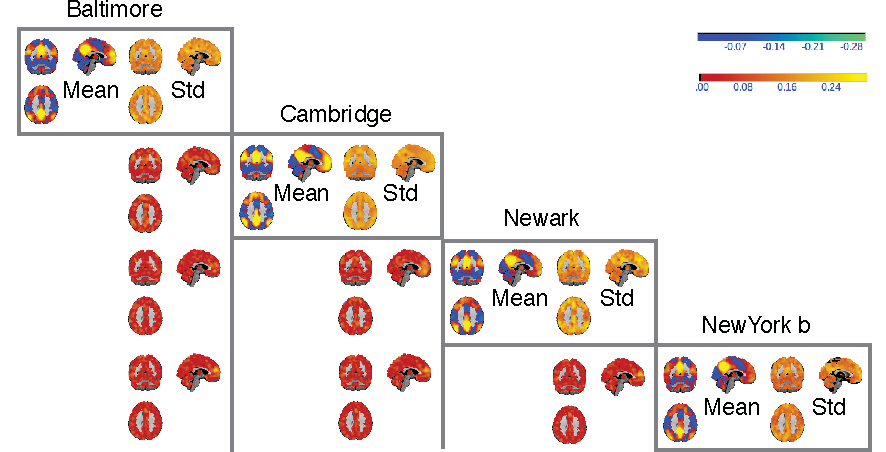
\includegraphics[width=\linewidth]{../figures/mult_center_dm_voxel_seed_3tonly.pdf}
\end{center}
\tiny{DMN variability across sites (Dansereau et al. article en préparation)
%Functional connectivity maps of the default-mode network at multiple sites. The average connectivity map for 4 sites (Baltimore, Cambridge, Newark and New-Yorkb at 3T) are presented on the diagonal (left). The standard deviation across subjects and within site is presented next to it (diagonal squares, right part). Each off-diagonal block represent the absolute difference between the average functional connectivity maps between two sites (called the inter-site bias).
}
\end{figure}
}

% \frame{
% \frametitle{Simulation: connectome}
% {Connectome}
% \begin{itemize}
% \item On calcul un connectome a partir d’une partition en $R$
%  reseaux.
% \item la connectivité inter-reseaux $y_{i,j}$ est calculé par transformation Fisher la la corrélation de Pearson
% \item On obtient un connectome $R\times R$ symétrique
% \end{itemize}
% }

% \begin{frame}
% \frametitle{Connectivitée au repos}
% \begin{figure}
% \begin{center}
% \pgfimage[width=0.9\linewidth]{../figures/connectome.png}
% \end{center}
% \tiny{Bellec et al. Neuroimage 2006, connectome fonctionnel.}
% \end{figure}
% \end{frame}
%Using a brain partition of $R$ networks obtain from BASC procedure described in Bellec et al. 2010, and taking each pair of distinct networks $i$ and $j$, the between-network connectivity $y_{i,j}$ is measured by the Fisher transform of the Pearson's correlation between the average time series of the network. The within-network connectivity $y_{i,i}$ is the Fisher transform of the average correlation between time series of every pair of distinct voxels inside network $i$. The connectome $\mathbf{Y}=(y_{i,j})_{i,j=1}^R$ is thus a $R\times R$ matrix. Each column $j$ (or row, as the matrix is symmetric) codes for the connectivity between network $j$ and all other brain networks (full brain functional connectivity map). For a scale with $R$ parcels, there are exactly $L=R(R+1)/2$ distinct elements in an individual connectome $\mathbf{Y}$. 



\frame{
\frametitle{Simulation: correction multi-site (methode 1)}

Introduction de variables dites «dummy» dans le GLM.
%Depending on the multi-site configuration and distribution of the subject we proposed two corrective approaches that can be applied as shown in the simulations of Figure \ref{fig_simu_50pct}. The first one is the introduction of dummy variables (binary vectors $1\times N$) who code for each site in the GLM model \ref{dummy variable equation}.

%The variables are corrected to have a zero mean across subjects, and an intercept (i.e. a column filled with 1) is added to $\mathbf{X}$. The GLM relies on the following stochastic model:
 \begin{equation}
 \label{eq_glm}
  \mathbf{Y} = \mathbf{X}\mathbf{\beta} + \mathbf{V}\mathbf{\gamma}+ \mathbf{E},
 \end{equation}
 \begin{itemize}
  \item $\mathbf{Y}$: $N\times 1$, valeurs de connectivité pour la paire ($i,j$),
  \item $\mathbf{X}$: $N\times K$, variables explicatives,
  \item $\mathbf{\beta}$: $1 \times K$, valeurs de régression pour chaque variable explicative,
  \item $\mathbf{V}$: $N\times S$, chaque colonne code pour un site (0/1),
  \item $\mathbf{\gamma}$: $1\times S$, moyennes de connectivité par site,
  \item $\mathbf{E}$: $N\times 1$, résidus de la régression,
 \end{itemize}
avec $N$ nombre de sujets, $K$ nombre de variables explicatives, $S$ nombre de sites.
%where $\mathbf{\beta}$ is an unknown $C\times L$ matrix of linear regression coefficients and $\mathbf{E}$ is a $N\times L$ random (noise) multivariate Gaussian variable.
%To apply the correction $v-1$ dummy-variables are added to the model \ref{dummy variable equation} with $v$ being the total number of sites used in the study.

% \begin{equation}
%     y_{i,j} = \beta x+\beta_{i=1,\dots,v-1}x_{i=1,\dots,v-1}+e
%     \label{dummy variable equation}
% \end{equation}
}


\frame{
\frametitle{Simulation: correction multi-site (methode 2 METAL)}
%The second approach is to compute the GLM independently on each site and then combine the statistical results from each site in a global score. This model averaging technique called METAL from Willer 2010 model site specific bias by running a GLM analysis on each site resulting in $v$ beta vectors that are weighted proportionally to the standard error of each site and finally averaged as shown in equation. This is the most flexible way to account for multi-site effect wile keeping the analysis simple and robust to unbalanced sites.

\begin{equation}
	\beta_{v} \text{, effect size estimate for site \textit{v}.}
\end{equation}
\begin{equation}
	\sigma_{v} \text{, standard error for site} \textit{v}.
\end{equation}
\begin{equation}
 	w_{v}=\frac{1}{\sigma_{v}^{2}} \text{, weight estimate for site \textit{v}.}
 \end{equation}
 \begin{equation}
 	\beta=\frac{\Sigma_{v}\beta_{v}w_{v}}{\Sigma_{v}w_{v}} \text{, global }\beta.
 \end{equation}
  \begin{equation}
 	\sigma=\sqrt{\frac{1}{\Sigma_{v}w_{v}}} \text{, global standard error.}
 \end{equation}
\begin{equation}\label{METAL}
	Z=\frac{\beta}{\sigma} \text{, global Z score.}
\end{equation}
\begin{equation}
	p=2(1-\phi(\vert Z \vert) \text{, p-value.}
\end{equation}
}

% \frame{
% \frametitle{Résultats: ICC}
% %The Figure \ref{fig_icc} presents the results of the ICC analysis for the point-to-point correlations, only the connections with an average ICC above 0.5 are represented. The results were consistent with (Shehzad et al. 2009), with a mean ICC over all connections of \textasciitilde0.3 and 23 connections scoring a moderate-to-good level of ICC ($>0.5$). 
% 
% \begin{figure}
% \begin{center}
% 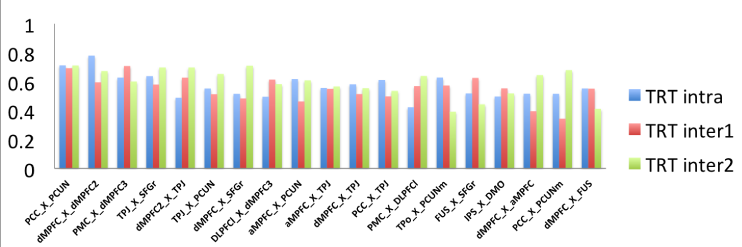
\includegraphics[width=\linewidth]{../figures/fig_icc.png}
% \end{center}
% \tiny{
%   ICC scores for pairs of connections passing the $>0.5$ threshold on the NYU-TRT dataset.
% }
% \end{figure}
% }

% \frame{
% \frametitle{Résultats: meta-analyse}
% \begin{figure}
% \begin{center}
% \pgfimage[width=0.8\linewidth]{../figures/fig_freq_sel_dat.png}
% \end{center}
% \tiny{
%   Frequency of reported regions showing functional differences based on a literature review of 6 papers.
% }
% \end{figure}
% }

% \frame{
% \frametitle{Résultats: parcèlles sélectionné dans le DMN}
% \begin{figure}
% \begin{center}
% \pgfimage[width=0.45\linewidth]{../figures/fig_nodes_DMN.png}
% \end{center}
% \tiny{
%   Selected nodes inside the DMN who passed the TRT selection.
% }
% \end{figure}
% }

% \frame{
% \frametitle{Résultats: parcèlles sélectionné à l'exterieur du DMN}
% \begin{figure}[H]
% \begin{center}
% \pgfimage[width=0.8\linewidth]{../figures/fig_nodes_non_DMN.png}
% \end{center}
% \tiny{
% 	  Selected nodes outside the DMN who passed the TRT selection.
% }
% \label{fig_nodes_none_DMN}
% \end{figure}
% }


% \frame{
% \frametitle{Résultats: pair de connection sélectionné}
% \begin{table}
% \begin{center}
% \resizebox{\columnwidth}{!}{%
% \begin{tabular}{l l l l}
% \bfseries{Network} & \bfseries{Label} & \bfseries{Name} & \bfseries{Cambridge100}\\
% \hline
%  & PCC & posterior cingulate cortex & 1\\
%  & dMPFC & dorsomedial prefrontal cortex & 12\\
%  & dMPFC2 & dorsomedial prefrontal cortex & 46\\
% Default-mode network & aMPFC & anterior medial prefrontal cortex & 42\\
%  & IPL & inferior parietal lobule & 49\\
%  & PCUN & precuneus & 53\\
%  & MTL & medial temporal lobe & 39\\
%  & SFGr & right superior frontal gyrus & 76\\
% \hline
% Visual network & FUS & fusiformgyrus & 71\\
% \hline
% Dorsal attentional & PCUMm & precuneus (motor) & 94\\
% \hline
% Cingulo-opercular network & dMPFC3 & dorsmedial prefrontal cortex & 90\\
% \end{tabular}
% }
% \end{center}
% \tiny{Regions selected in the literature review, the region number correspond to the number in the Cambridge 100 partition.}
% \end{table}
% }

% \frame{
% \frametitle{Résultats: pair de connection sélectionné}
% For point-to-point correlations within the DMN, we selected the connections with highest ICC for each node (all average $ICC > 0.5$):
% \begin{itemize}
% \item PCC x PCUN
% \item dMPFC x dMPFC2
% \item IPL x SFGr
% \item aMPFC x PCUN
% \end{itemize}
% For each point-to-point correlation between the DMN and another network, we selected the connections with highest ICC and $ICC > 0.5$:
% \begin{itemize}
% \item FUS x SFGr
% \item PCC x PCUNm
% \item IPL x dMPFC3
% \end{itemize}
% }
%
%\frame{
%\frametitle{Résultats: STD inter vs. intra}
%%The first assessment perform on the dataset was to verify the distribution of the variance in functional connectivity among each site and across sites in order to see if they are of the same order of magnitude or not. This analysis of Figure \ref{fig_site_variability} shows the distribution of the standard deviation of connectivity across subjects (the distribution is over the full brain connectome, with several 1000s connections) at the 8 sites against the inter-sites standard deviation of connectomes (average at each site). as we can see the inter-site (between site) variability is smaller than the intra-site (between subjects) variability.
%
%\begin{figure}
%\begin{center}
%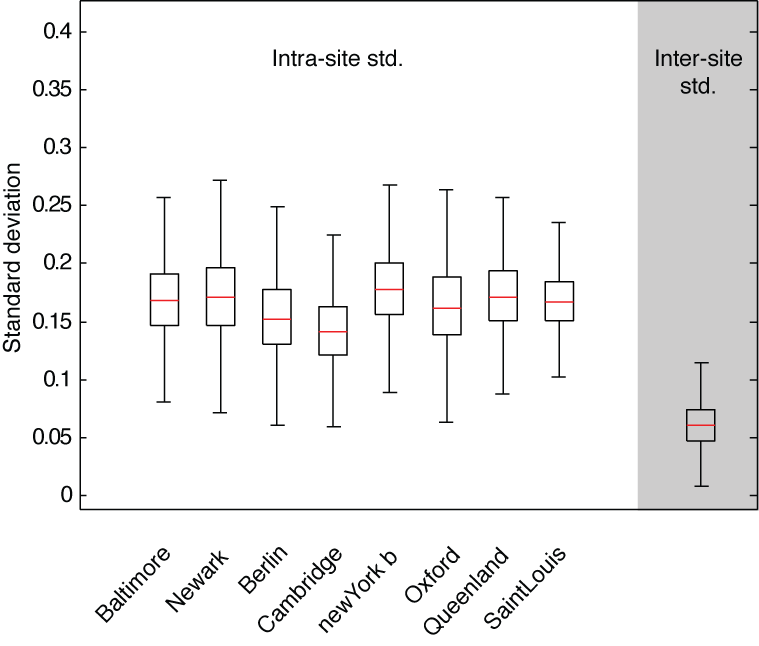
\includegraphics[width=0.7\linewidth]{../figures/inter_vs_intra_3tonly.png}
%\end{center}
%\tiny[inter vs. intra site variability]{
%  Distribution of intra-site (between-subject) standard deviation vs. inter-site (between-site) standard deviation, based on the standard deviation of the connectivity matrices from 8 sites from the 1000 functional connectome dataset.
%}
%\end{figure}
%}

%\frame{
%\frametitle{Résultats: pouvoir de détection}
%%We also showed using Monte-Carlo simulations that the power of detecting an effect is marginally affected by the site acquisition configuration (single site or multi-site, see Figure3.2 for an illustration of a power analysis on three different seeds) where the sites are balanced in term of the amount of subject with and without the effect. 
%
%\begin{figure}
%\begin{center}
%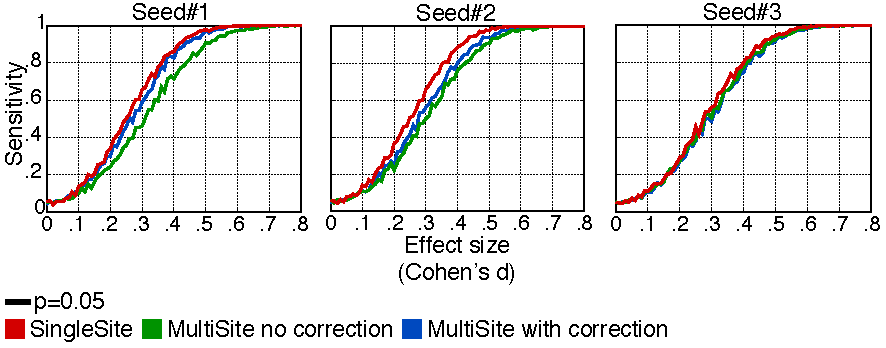
\includegraphics[width=\linewidth]{../figures/simu_results_multisite.pdf}
%\end{center}
%\tiny[Detection power]{
%Power analysis for a resting-state fMRI study. A Monte-Carlo simulation was implemented to evaluate the power of a resting-state multi-site study, based on real values of three connections in the default-mode network PCC/MFC, rHIP/vMFC and lIPC-rDLPFC. For each site and each sample, half of the subjects were randomly assigned to a 'treatment' group. For the subjects in this group, a value was added to achieve a given relative effect size (Cohen's d, i.e. the mean of the two groups divided by the standard deviation of all sites). The significance of the difference between the control and 'treatment' group was assessed by a $t$-test in a linear model, including covariates to model site-specific bias. The study was repeated for various effect sizes (0 to 0.8 with a step of 0.01) at a threshold of 0.05 on the p-value in the $t$-test. For a p of 0.05, a statistical power of 0.
%95 can be achieved for as low as a 0.47 effect size. The simulation was based on a scenario with 8 sites and 385 subjects, and no homogeneization of acquisition protocol whatsoever. The multi-site (with and without correction) is based on 187 subjects from 7 sites and the SingleSite is based on one site of 198 subjects. 
%}
%\label{fig_detection_power}
%\end{figure}
%}

\frame{
\frametitle{Simulation: cohen's d}
Pour chaque site, un effet est ajouté à la connectivité de 50\% des sujets, sélectionnés aléatoirement (groupe «pathologique»):
%Pour chaque site, 50\% des sujets sont assignés au groupe «traitement» de manière aléatoire et une simulation Monte-Carlo est utilisé pour estimer le pouvoir de détection (en mono-site et en multi-site)
\begin{equation}
	y_{i,j} = y_{i,j} + \mu.
\end{equation}

%The normalized Cohen's d was used to estimate the effect size and it is defined as the difference between two means $\bar{x_{1}},\bar{x_{2}}$ divided by a standard deviation from the data $s$.
Le paramètre $\mu$ est choisi pour réaliser une certaine taille d'effet (mesuré par le $d$ de Cohen): %(difference entre deux moyenne $\bar{x_{1}},\bar{x_{2}}$) divisé par la deviation standard $s$.
\begin{equation}\label{cohen's d}
    \begin{array}{l l}
      d = \frac{\mu}{s_{i,j}},      
    \end{array}
\end{equation}
où $s_{i,j}$ est l'écart-type de la connectivité entre les régions $i$ et $j$ pour la population de référence (mono-site, Cambridge). Différentes tailles d’effet sont simulées (de 0 à 0.8). 


%$n_{1}$ and $n_{2}$ are the respective number of subject in each group. In order to introduce the same effect-size across the single-site and multi-site dataset we are taking the standard deviation from the single-site cohort as the reference.  The connection $y_{i,j}$ of the randomly affected subjects ("treatment" group) are therefore calculated $y_{i,j} = y_{i,j} + d\times s_{i,j}$. The significance of the difference between the control and 'treatment' group was assessed by a $t$-test in a linear model, including a covariate to model the motion. The study was repeated for various effect sizes (0 to 0.8 with a step of 0.01) with a $p$-value threshold of $0.05$ on the $t$-test.
}

\frame{
\frametitle{Résultats: pouvoir de détection avec les deux corrections}
\begin{figure}
\begin{center}
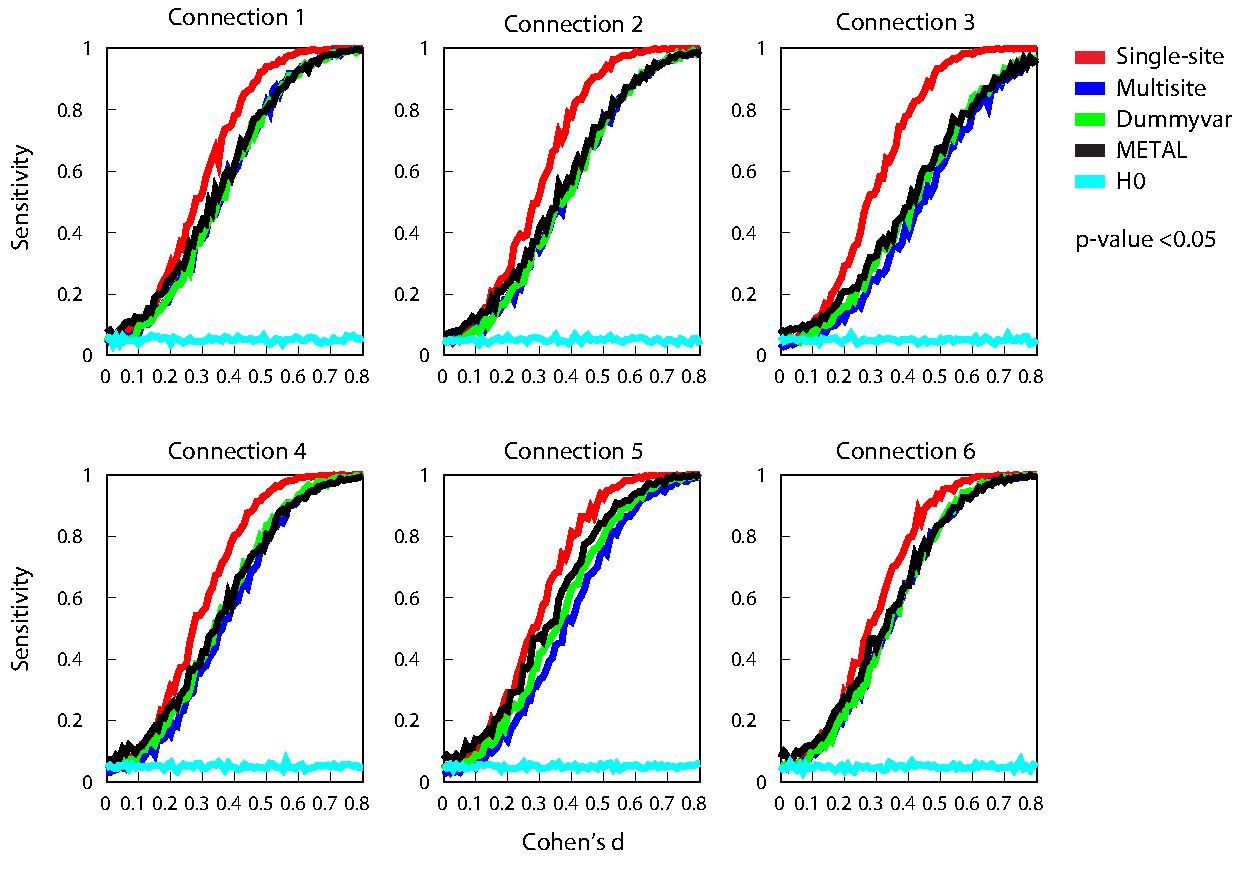
\includegraphics[width=0.9\linewidth]{../figures/multisite_simulation_50pct.pdf}
\end{center}
\tiny{Pouvoir de détection  (Dansereau et al. article en préparation)
%Power analysis for a resting-state fMRI study. A Monte-Carlo simulation was implemented to evaluate the power of a resting-state multi-site study. For each site and each sample, half of the subjects were randomly assigned to a 'treatment' group. For the subjects in this group, a value was added to achieve a given relative effect size (Cohen's d, i.e. the mean of the two groups divided by the standard deviation of all sites). The significance of the difference between the control and 'treatment' group was assessed by a $t$-test in a linear model. To correct for site-specific bias two correction are presented the dummy variables and METAL. The study was repeated for various effect sizes (0 to 0.8 with a step of 0.01) at a threshold of 0.05 on the p-value in the $t$-test. The simulation was based on a scenario with 8 sites and 385 subjects, and no homogeneization of acquisition protocol whatsoever. The multi-site (with and without correction) is based on 187 subjects from 7 sites and the Single-site is based 
%on one site of 198 subjects. 
}
\end{figure}
}

\frame{
\frametitle{Étude multi-sites conclusion}
\begin{itemize}
\item Existence d’un biais multi-sites.
\item Selon la répartition des sujets, on peut avoir une petite diminution du pouvoir statistique.
\item A compléter: exploration de scénarios plus complexes (sites débalancés, petits sites).

\end{itemize}
}
%We confirmed that multi-site acquisition introduce some variability in the dataset although a single-site study with 200 subjects had only a marginally superior statistical power than an analysis pooling 7 sites for an equivalent number of subjects. In both cases, a high sensitivity ($>0.95$) could be achieved for the effect size observed by Goveas 2011 which reported an effect equivalent to 1. We can therefore conclude that it is feasible to acquire rs-fMRI data in across multiple sites and correct for this topology.
%\end{document}
%------------------------------------------------

%------------------------------------------------
\section{Classification et analyse multivariée} 
%------------------------------------------------
\frame{\sectionpage}
% 
% \frame{
% \frametitle{Connectome et reduction de l'espace}
% \begin{itemize}
% \item Métric standard Pearson correlation ($n\times n$) matrice de connectivité de chaque voxel dans la matiere grise
% \item Il y a approximativement $10^4$ voxels dans la matière grise
% \item $5\times10^7$ connections possible a exploré
% \item Petit nombre de sujets $<10^3$ (exemple)
% \item Même SVM ne se comporte pas bien dans un cas de ce genre
% \item On tire parti de la structure des données pour réduire la dimension du problème (connectome multi échelle)
% \end{itemize}
% }

\begin{frame}
\frametitle{Connectivitée au repos}
\begin{figure}
\begin{center}
\pgfimage[width=0.9\linewidth]{../figures/connectome.png}
\end{center}
\tiny{Bellec et al. Neuroimage 2006, connectome fonctionnel.}
\end{figure}
\end{frame}

\begin{frame}
\frametitle{Décomposition en réseaux}
\begin{figure}
\begin{center}
\pgfimage[width=0.5\linewidth]{../figures/CRSN.png}
\end{center}
\tiny{Dansereau et al. 2014 Front. Neurosci. in press.}
\end{figure}
\end{frame}
%Once the data is preprocessed properly, we need to derive some metric of brain connectivity. One of the most common metric is the Pearson correlation, and is usually represented as a $n\times n$ connectivity matrix of every voxel in the gray matter. As there are in the order of $10^4$ voxels, there is an overwhelming number of $5\times10^7$ possible connections to examine as a potential diagnostic tool. We therefore have a very large number of features, but only few of them are potentially relevant for diagnostic purposes. Unfortunately, only a quite limited number of examples are available in a typical neuroimaging study to learn which connections are the most informative ($<10^3$). Even state-of-the-art classification algorithms (e.g. SVM Cortes1995) cannot overcome the presence of large number of weakly relevant and redundant features. This is usually attributed to "the curse of dimensionality" (Bellman1961), or to the fact that irrelevant features decrease the ability of the learner to discriminate 
%between classes. Moreover, many machine-learning algorithms become computationally intractable when the dimension is high. On the other hand once a reduce set of features has been chosen even the most basic classifiers can achieve high performance classification.

%In order to reduce that feature space and to have a clinically meaningful representation of functional structures, a number of solutions have been proposed that take advantage of the underlying structure of the brain (Heuvel2009). Regions are routinely defined using an anatomical parcellation (He2009), such as the AAL template (Tzourio-Mazoyer2002. Anatomical parcels may however not well match the organization of resting-state networks. We use a framework to generate data-driven functional decomposition into resting-state networks based on the coherence of fMRI time series at the individual or group level (Bellec2006,Bellec2010c). When a low number of networks (or scale) are used, this technique, called bootstrap analysis of stable clusters (BASC), generates decompositions of the brain into distributed large-scale networks, such as the default mode network (DMN). At high scales, it identifies sub-networks and functional regions (Kelly2012). We can therefore use those parcellation units to reduce the feature 
%space.


\frame{
\frametitle{Connectomes multiéchelles}
\begin{figure}
\pgfimage[width=0.8\linewidth]{../figures/fig_connectome_multiscale}\\
\end{figure}
\tiny{Bellec et al., International Conference on Resting-state Connectivity, Magdeburg, 2012}
}
% 
% \frame{
% \frametitle{Métrique de stabilité}
% \begin{itemize}
% \item Corrélation est très utilisée, mais comporte beaucoup de variabilité.
% \item Investiguer d’autre métrique potentiellement moins sensible au mouvement aux artefacts d’acquisition.
% \item Stabilité (Bellec et al., 2010) «evidence accumulation of clustering on bootstrap samples».
% \item Évaluation des performances de la stabilité avec mon modèle de simulation de multi-sites.
% \end{itemize}
%Correlation is a good approach to asses connectivity but can be highly variable in noisy dataset. This motivated me to investigate another metric called "stability" based on evidence accumulation of clustering on bootstrap samples, that could potentially be more consistent across subjects and scanning session resulting in improved prediction power and generalizability. The stability metric was design in an attempt to reduce the variance in the acquisition and extract the most consistent functional structures in the underling data by bootstrapping temporal blocks to identify the regions that are most often clustered together even though the temporal block are re-sampled. In an attempt to extend my current work I will use the simulations that I have design to evaluate the multi-site effect (1000 functional connectome dataset composed of one large site and 7 smaller sites) in order to evaluate if the detection power is improved or not using a stability metric instead of a correlation metric and if it is robust 
%to various multi-site scenarios.
}

% \frame{
% \frametitle{Identification des «features» et du classifieur}
% \begin{itemize}
% \item Identification des connexions les plus discriminantes.
% \item Tenir compte des variables confondantes (age, sexe, éducation, multi-sites, mouvement).
% \item Stabilité des connexions choisies (échantilonage bootstrap).
% \item 10-fold cross-validation (performance de classification).
% \item Matrices multi-échelles et interactions inter-échelle (apprentissage de la réduction de donnée optimale).
% \item Combinaison de techniques standards (Linear Discriminant Analysis (LDA), SVM , AdaBoost) avec de nouvelle méthodes de sélection de «features».
% \end{itemize}
% %A crucial point of our study is to identify the most discriminant features to use in the prediction model and account for various confounding factors (e.g. age, gender, education, multi-site effect and motion). This is future work that will be conducted in the next year and a half. I will particularly focus on the stability of the features selected, in order to obtain robust and consistent markers of the disease. In order to estimate stability of the selection I plan to use a Monte-Carlo estimation of the selection using bootstrap resampling (Efron1994,Bellec2010c) on the training dataset inside a 10-fold cross-validation. The large feature space that will be fed to this procedure will be a correlation matrix of network at multiple scales. As an example, let's take 3 parcellations (e.g. scales 10, 50, 100) of the functional brains obtained from an independent dataset of normal subjects using the method describe in the previous section (Large feature space). Using the time-series of every parcellation I will 
% %obtain a correlation matrix $A$ of size $R\times R$ and $R=10+50+100=160$ resulting in a vectorized form of this matrix of size $L=R(R+1)/2=12880$ unique features. The idea behind this strategy is to capture interaction of small networks with larger networks instead of just looking at the interaction of large network with large network or small network with small network which could miss some important interaction. An example of previously mentioned interaction of larger network with smaller ones is the known decrease in connectivity between the hippocampal structure (small regions) with the default mode (a large and extended network). This procedure could potentially capture those interactions that would in term maximize the prediction accuracy as well as controlling for stability by only retaining the most stable features identified by the feature selection therefore enforcing generalizability. Venkataraman et al. 2010 as used stability measures with Gini importance metric and found a good performance 
% %distinguishing between patients with schizophrenia and normal control.
% 
% %More work also needs to be done in finding the appropriate classification method and investigating several standard alternatives in conjunction with novel feature selection methods will also be part of my project in the next year. I will notably consider the Linear Discriminant Analysis (LDA) because it is straightforward to include covariates in the model in order to account for confounding effects. I will also evaluate SVM since it is a very popular method, and I will more particularly investigate the margin optimisation criteria for feature selection (Gilad-bachrach 2004,Kononenko1997). One last approach will be to use ensemble techniques like AdaBoost (Freund et al. 1997 to improve generalization performance. AdaBoost as been proved to be remarkably resistant to overfitting (Schapire 1998). An interesting point is that Schapire et al. 1998 has shown using a slightly different definition of the margin that AdaBoost also "boosts" the margins, meaning that it finds the decision boundary that is further 
% %away from the instances of all classes. By margin Schapire refers to the difference between the total vote AdaBoost receives from correctly identifying classifiers and the maximum vote received by any incorrect class. 
% }
% 
\frame{
\frametitle{Évaluation du pipeline et plan d’analyse}
\begin{enumerate}
\item Cobre (74 controles, 72 schizophrénes).
\begin{itemize}
\item Prédiction de la maladie.
\end{itemize}
\item Enhanced Nathan Kline Institute-Rockland Sample (NKI) ($>500$ subjects).
\begin{itemize}
\item Prédiction de l’âge.
\item Multi protocoles.
\end{itemize}
\end{enumerate}


%The evaluation of the classification pipeline will be done using two datasets namely: 1) the Cobre dataset composed of 74 control and 72 schizophrenic subjects and 2) the enhanced Nathan Kline Institute-Rockland Sample (NKI-RS) a large community sample representing $>500$ subjects. The Cobre dataset will be use to study the ability of the method to identify discriminative features of schizophrenia (previous univariate analysis have shown large effect on the same dataset). We will also use the NKI-RS to predic the effect of age. Another interesting aspect of the NKI-RS is that every subject has been scanned with different fMRI protocol (scanner parameters) on the same scanner. We can use this information to have a pseudo multi-site data set and explore the generalization of the trained classifier on the same  with a different scanning protocol.
}

\frame{
\frametitle{Implication dans l'industrie}
\begin{itemize}
\item Consultation pour des sous-traitants de pharmaceutique (NeuroRx et Biospective).
\item Preuve de faisabilité et analyses pour des essais clinique de phase II sur la maladie d’Alzheimer pour le compte de grand joueur de l'industrie pharmaceutique.
\item Identification de biomarqueur avec le Canadian Consortium on Neurodegeneration in Aging (CCNA).
\end{itemize}
%I am involved in the industry (through my consulting work with the companies NeuroRX and Biospective), I'm advising on the fMRI analysis of multiple clinical trials and looking at the feasibility of using fMRI in multicentric pharmaceutical trials (some of these work have lead to publications). I'm also doing statistical analysis and proposing biomarkers tailored to the clinical questions of the pharmaceutical sponsors. I'm also starting to get involved with the biomarker unit of the Canadian Consortium on Neurodegeneration in Aging (CCNA) who wants to propose new biomarker for Alzheimer disease that would be use systematically in the clinical assessment of Alzheimer disease across Canada. These efforts and collaborations are perfectly in line with the objectives of my PhD. and are greatly contributing to translational findings and application of my research in pharmaceutical trials as well as addressing concrete question in the field of neuroimaging.
}

\frame{
\frametitle{Timeline}
J’ai identifié trois questions que je compte adresser dans mon PhD:
\begin{itemize}
\item Impact du mouvement sur la connectivité (posters présentés à OHBM2013 et AAIC2014 article en préparation soumis avant la fin de l'hiver 2015).

%Investigate motion impact on functional connectivity I'm currently writing a manuscript that should be submitted at the end of this year (2014) on that specific topic. The results have been presented (poster format) at the Organization for Human Brain Mapping conference 2013 (OHBM) and at the Alzheimer's Association International Conference 2014 (AAIC).

\item Faisabilité d'étude multi-sites (poster présentés à OHBM2013 et AAIC2013 article en préparation soumis avant l'été
 2015).
%\item Feasibility of multi-site connectivity analysis (inter-site normalization) Most of the analyses are completed and some of the results have been presented in two conferences (poster format), namely OHBM2013 and AAIC2013. I'm planning to submit the manuscript for this study mid 2015.

\item Prediction 
\begin{itemize}
\item Expérimenter avec les outils d’apprentissage et identifier des métriques à utiliser.
\item Faire une validation de la stabilité.
%\item I'm currently experimenting with some standard machine learning tools and I will start by testing the pipeline on simple simulations and verify is the stability metric is more resistant to structured noise.
\item Application sur données réelles avec Cobre et NKI-RS.
%\item  Then on a real dataset I will apply the pipeline on Cobre and NKI-RS.
\item Évaluation du pipeline sur un jeu de données final (5 sites) en cross sectionnel et 1 site en longitudinal (prendre fin à l'hiver 2016).
%\item Finally I will apply the pipeline on a dataset that I have compiled in the past year, this dataset is composed of 313 elderly adults with and without cognitive impairment of the Alzheimer type collected across 5 studies: ADNI2 study and 4 other studies based in Montreal, Canada, for a grand total of 126 CNE participants, 133 patients with MCI, and 54 patients with DAT. I will try to classify the various population in a cross sectional analysis. I am also planning to use a subset of the data namely the ADNI2 dataset who is a longitudinal study to assess the potential of the method to predict time of conversion from pMCI to pDAT. I plan to be done with those analyses in the winter of 2016 and publish the results in the following months.

\end{itemize}

\item Je planifie soumettre ma thèse à la fin 2016.
%\item Finally I plan to submit my theses at the end of 2016 (see Timeline \ref{timeline})

\end{itemize}
}

%------------------------------------------------

%\begin{frame}
%\frametitle{Future work}
%\end{frame}

%------------------------------------------------

% Time line
%------------------------------------------------

%\frame{
%\frametitle{Time line}
% \begin{table}
% \begin{tabular}{lllllllll}
% & \multicolumn{2}{l}{2013}& \multicolumn{2}{l}{2014}& \multicolumn{2}{l}{2015}& \multicolumn{2}{l}{2016}\\
% Motion & \cellcolor{black!25}& \cellcolor{black!25}&  \cellcolor{black!25}& \cellcolor{black!25}& & & & \\
% Multisite & \cellcolor{black!25}& \cellcolor{black!25}&  \cellcolor{black!25} & \cellcolor{black!25}& \cellcolor{black!25}& & & \\
% Prediction & & & & \cellcolor{black!25}& \cellcolor{black!25}&  \cellcolor{black!25}& \cellcolor{black!25}& \\
% Theses & & & & & & & & \cellcolor{black!25} \\
% \end{tabular}
% \end{table}
%}

%------------------------------------------------

\begin{frame}
\Huge{\centerline{Merci}}
\end{frame}

%----------------------------------------------------------------------------------------

%\begin{frame}
%\frametitle{Blocks of Highlighted Text}
%\begin{block}{Block 1}
%Lorem ipsum dolor sit amet, consectetur adipiscing elit. Integer lectus nisl, ultricies in feugiat rutrum, porttitor sit amet augue. Aliquam ut tortor mauris. Sed volutpat ante purus, quis accumsan dolor.
%\end{block}
%
%\begin{block}{Block 2}
%Pellentesque sed tellus purus. Class aptent taciti sociosqu ad litora torquent per conubia nostra, per inceptos himenaeos. Vestibulum quis magna at risus dictum tempor eu vitae velit.
%\end{block}
%
%\begin{block}{Block 3}
%Suspendisse tincidunt sagittis gravida. Curabitur condimentum, enim sed venenatis rutrum, ipsum neque consectetur orci, sed blandit justo nisi ac lacus.
%\end{block}
%\end{frame}

%------------------------------------------------

%\begin{frame}
%\frametitle{Multiple Columns}
%\begin{columns}[c] % The "c" option specifies centered vertical alignment while the "t" option is used for top vertical alignment
%
%\column{.45\textwidth} % Left column and width
%\textbf{Heading}
%\begin{enumerate}
%\item Statement
%\item Explanation
%\item Example
%\end{enumerate}
%
%\column{.5\textwidth} % Right column and width
%Lorem ipsum dolor sit amet, consectetur adipiscing elit. Integer lectus nisl, ultricies in feugiat rutrum, porttitor sit amet augue. Aliquam ut tortor mauris. Sed volutpat ante purus, quis accumsan dolor.
%
%\end{columns}
%\end{frame}

%------------------------------------------------
%\section{Second Section}
%%------------------------------------------------

%\begin{frame}
%\frametitle{Table}
%\begin{table}
%\begin{tabular}{l l l}
%\toprule
%\textbf{Treatments} & \textbf{Response 1} & \textbf{Response 2}\\
%\midrule
%Treatment 1 & 0.0003262 & 0.562 \\
%Treatment 2 & 0.0015681 & 0.910 \\
%Treatment 3 & 0.0009271 & 0.296 \\
%\bottomrule
%\end{tabular}
%\caption{Table caption}
%\end{table}
%\end{frame}

%------------------------------------------------

%\begin{frame}
%\frametitle{Theorem}
%\begin{theorem}[Mass--energy equivalence]
%$E = mc^2$
%\end{theorem}
%\end{frame}

%------------------------------------------------

%\begin{frame}[fragile] % Need to use the fragile option when verbatim is used in the slide
%\frametitle{Verbatim}
%\begin{example}[Theorem Slide Code]
%\begin{verbatim}
%\begin{frame}
%\frametitle{Theorem}
%\begin{theorem}[Mass--energy equivalence]
%$E = mc^2$
%\end{theorem}
%\end{frame}\end{verbatim}
%\end{example}
%\end{frame}

%------------------------------------------------

%\begin{frame}
%\frametitle{Figure}
%Uncomment the code on this slide to include your own image from the same directory as the template .TeX file.
%%\begin{figure}
%%\includegraphics[width=0.8\linewidth]{test}
%%\end{figure}
%\end{frame}

%------------------------------------------------

%\begin{frame}[fragile] % Need to use the fragile option when verbatim is used in the slide
%\frametitle{Citation}
%An example of the \verb|\cite| command to cite within the presentation:\\~
%
%This statement requires citation \cite{p1}.
%\end{frame}

%------------------------------------------------

%\begin{frame}
%\frametitle{References}
%\footnotesize{
%\begin{thebibliography}{99} % Beamer does not support BibTeX so references must be inserted manually as below
%\bibitem[Smith, 2012]{p1} John Smith (2012)
%\newblock Title of the publication
%\newblock \emph{Journal Name} 12(3), 45 -- 678.
%\end{thebibliography}
%}
%\end{frame}



\end{document} 